% ---------------------------------------------------------------------------- %
\subsection{Versuch 3.1.1 -- Tr\"agheitsmoment $I_0$ des Pendels ohne Reiter}
\label{subsec:i0}
% ---------------------------------------------------------------------------- %

\begin{figure}[h!]
    \centering
    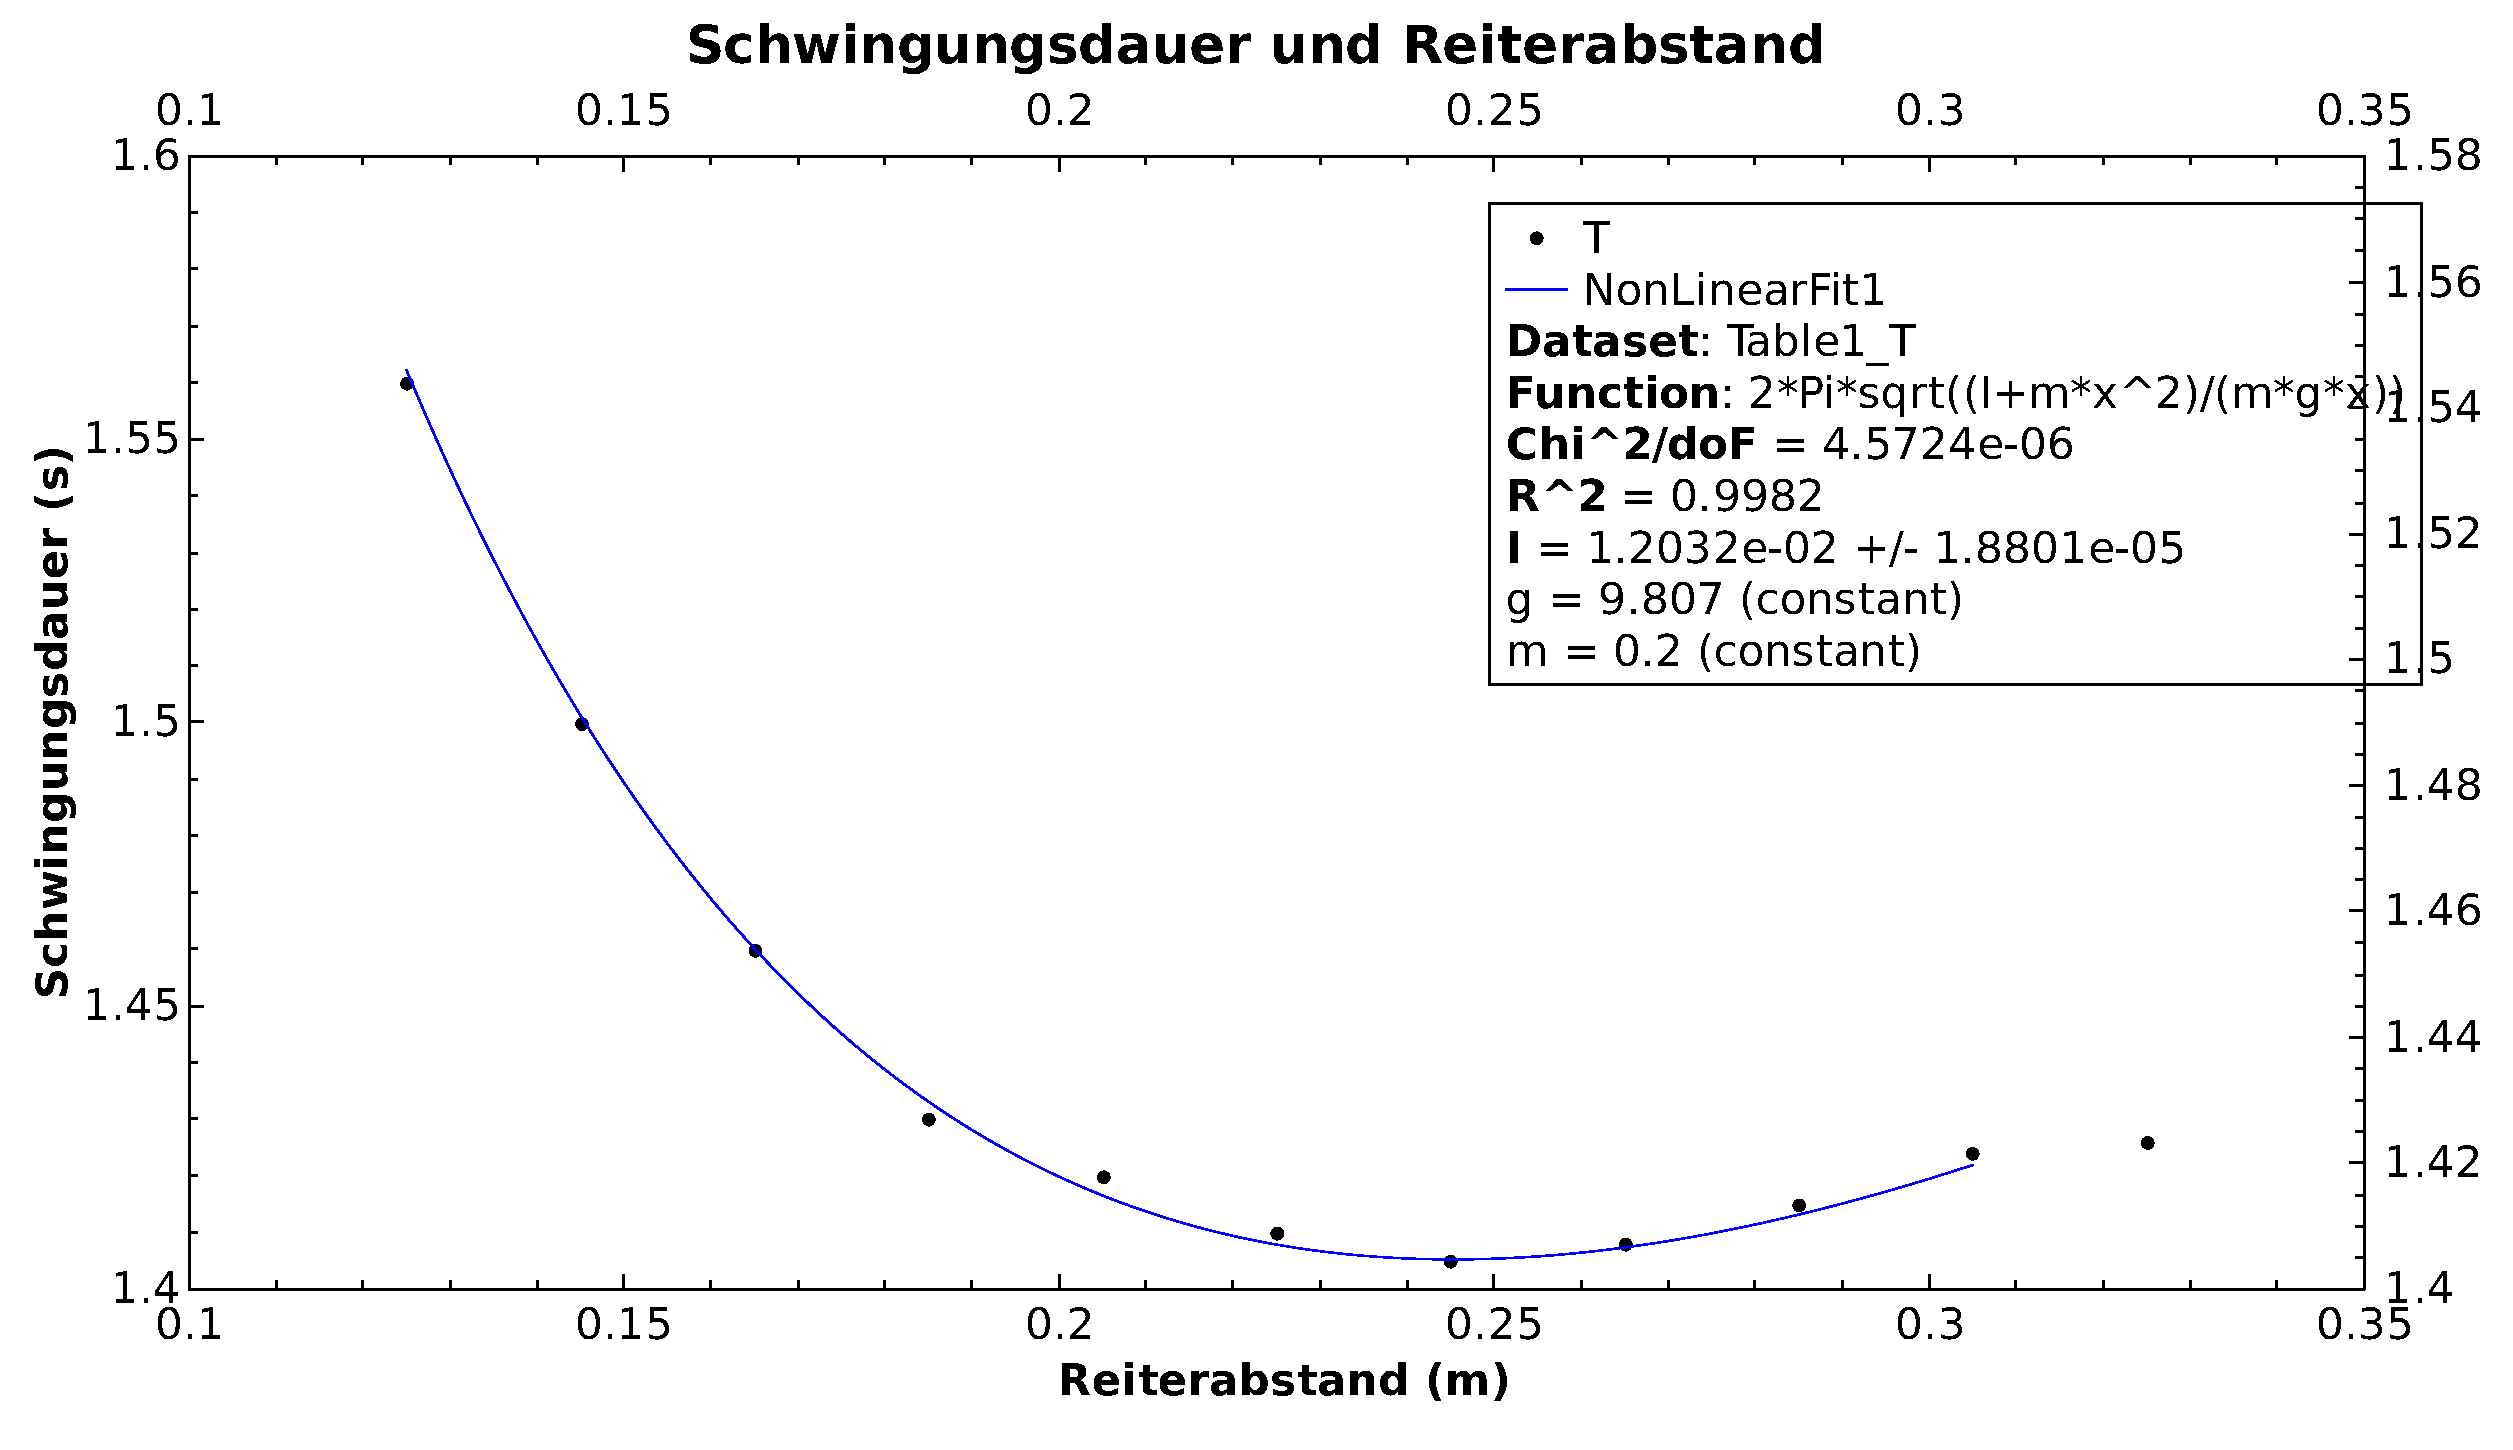
\includegraphics[width=\textwidth]{images/311.pdf}
    \caption{%
        Massentr\"agheitsmoment des Pendels ohne Reiter
    }
    \label{fig:pendelKonfigs}
\end{figure}

Die Messungen  wurden ausgef\"uhrt  mit einer Reitermasse  von \SI{200}{\gram}
und verschiedenen Abst\"anden. Der letzte Messpunkt bei \SI{325}{\milli\meter}
wurde  im  Fit nicht  ber\"ucksichtigt,  da  er  stark nach  einem  Ausreisser
aussieht.

Der Referenzwert aus der Versuchsanleitung f\"ur $I_0$ ist $\SI{1.16e-2}{\kilo\gram\meter\squared}$,
der mittels Fit ermittelte Wert betr\"agt $I_0  = \SI[separate-uncertainty = true]{12.032 \pm 0.018801}{\gram\meter\squared}$.


% ---------------------------------------------------------------------------- %
\clearpage
\subsection{Versuch 3.1.2 -- Schwingungsdauer in Funktion der Reitermasse}
\label{subsec:periodeReitermasse}
% ---------------------------------------------------------------------------- %

Im  Gegensatz zum  vorigen Versuch,  bei  dem die  Reitermasse als  Punktmasse
approximiert  wurde, sollte  gem\"ass Versuchsanleitung  das Tr\"agheitsmoment
des Reiters ab \SI{400}{\gram} ber\"ucksichtigt werden.

Da wir  in dieser Versuchsreihe  bis zu einer Reitermasse  von \SI{700}{\gram}
gemessen  haben, ist  es  naheliegend, eine  genauere Formel  herzuleiten. Ein
Problem beim  Fitten mit  QtiPlot in  diesem Fall, ist,  dass die  L\"ange des
Reiters mit  seiner Masse  variiert; man hat  also eigentlich  zwei Variablen,
welche sich  von Messung zu Messung  \"andern und in die  resultierende Formel
einfliessen sollten.

\begin{equation}
    T_0 = 2 \cdot \pi \cdot \sqrt{\frac{I_0 + I_{Reiter}}{m \cdot g \cdot a}}
\end{equation}

mit  $I_{Reiter}  =  I_{Zylinder} +  I_{Steineranteil}$. Mit  $I_{Zylinder}  =
\frac{m}{12} \cdot (  3 \cdot r^2 + h^2)$ und  $I_{Steineranteil} = m_{Reiter}
\cdot a^2$ (Quelle: Kuchling) ergibt dies:

\begin{equation}
    T_0 = 2 \cdot \pi \cdot \sqrt{\frac{I_0 + \frac{m_{Reiter}}{12} \cdot (3\cdot r^2 + h^2) + m_{Reiter} \cdot a^2}{m_{Reiter} \cdot g \cdot a}}
\end{equation}

Gl\"ucklicherweise  h\"angt  aber die  Masse  des  Reiters linear  von  seiner
L\"ange  ab (der  Durchmesser  aller Messproben  ist  identisch und  betr\"agt
\SI{34.4}{\milli\meter}); man hat also  nur einen Freiheitsgrad. Alles, was zu
tun bleibt, ist,  obige Gleichung in Funktion der  Zylinderl\"ange des Reiters
umzuschreiben, und den Fit mittels dieser Werte zu machen.

Dazu  wird  die   L\"angendichte  $\rho$  des  Reiters   als  neuer  Parameter
eingef\"uhrt, und  obige Funktion  umgeschrieben mit der  L\"ange $l_{Reiter}$
als  Funktionsparameter,   wobei  die  Reitermasse  dann   definiert  ist  als
$m_{Reiter} = \rho \cdot l_{Reiter}$:

\begin{equation}
    T_0 = 2 \cdot \pi \cdot \sqrt{\frac{I_0 + \frac{\rho \cdot l_{Reiter}}{12} \cdot (3\cdot r^2 + l_{Reiter}^2) + \rho \cdot l_{Reiter} \cdot a^2}{\rho \cdot l_{Reiter} \cdot g \cdot a}}
\end{equation}

Die verwendeten Parameter sind:
\begin{itemize}
    \item
        $\rho = \SI{6.667}{\kilo\gram\per\meter}$
    \item
        $l_{Reiter}$: Variable auf horizontaler Achse
    \item
        $r = \SI{17.2}{\milli\meter}$ (Radius des Reiters)
    \item
        $a = \SI{325}{\milli\meter}$ (Position des Mittelpunktes des Reiters)
    \item
        $g = \SI{9.807}{\meter\per\second\squared}$
\end{itemize}


Approximiert  man  den Reiter  als  Punktmasse  wie beim  vorherigen  Versuch,
ergibt   sich   das  Resultat   aus   Abbildung   \ref{fig:312a},  mit   einem
Massentr\"agheitsmoment von
$I_0  = \SI[separate-uncertainty = true]{11.362 \pm 0.39697}{\gram\meter\squared}$.
\begin{figure}[h!]
    \centering
    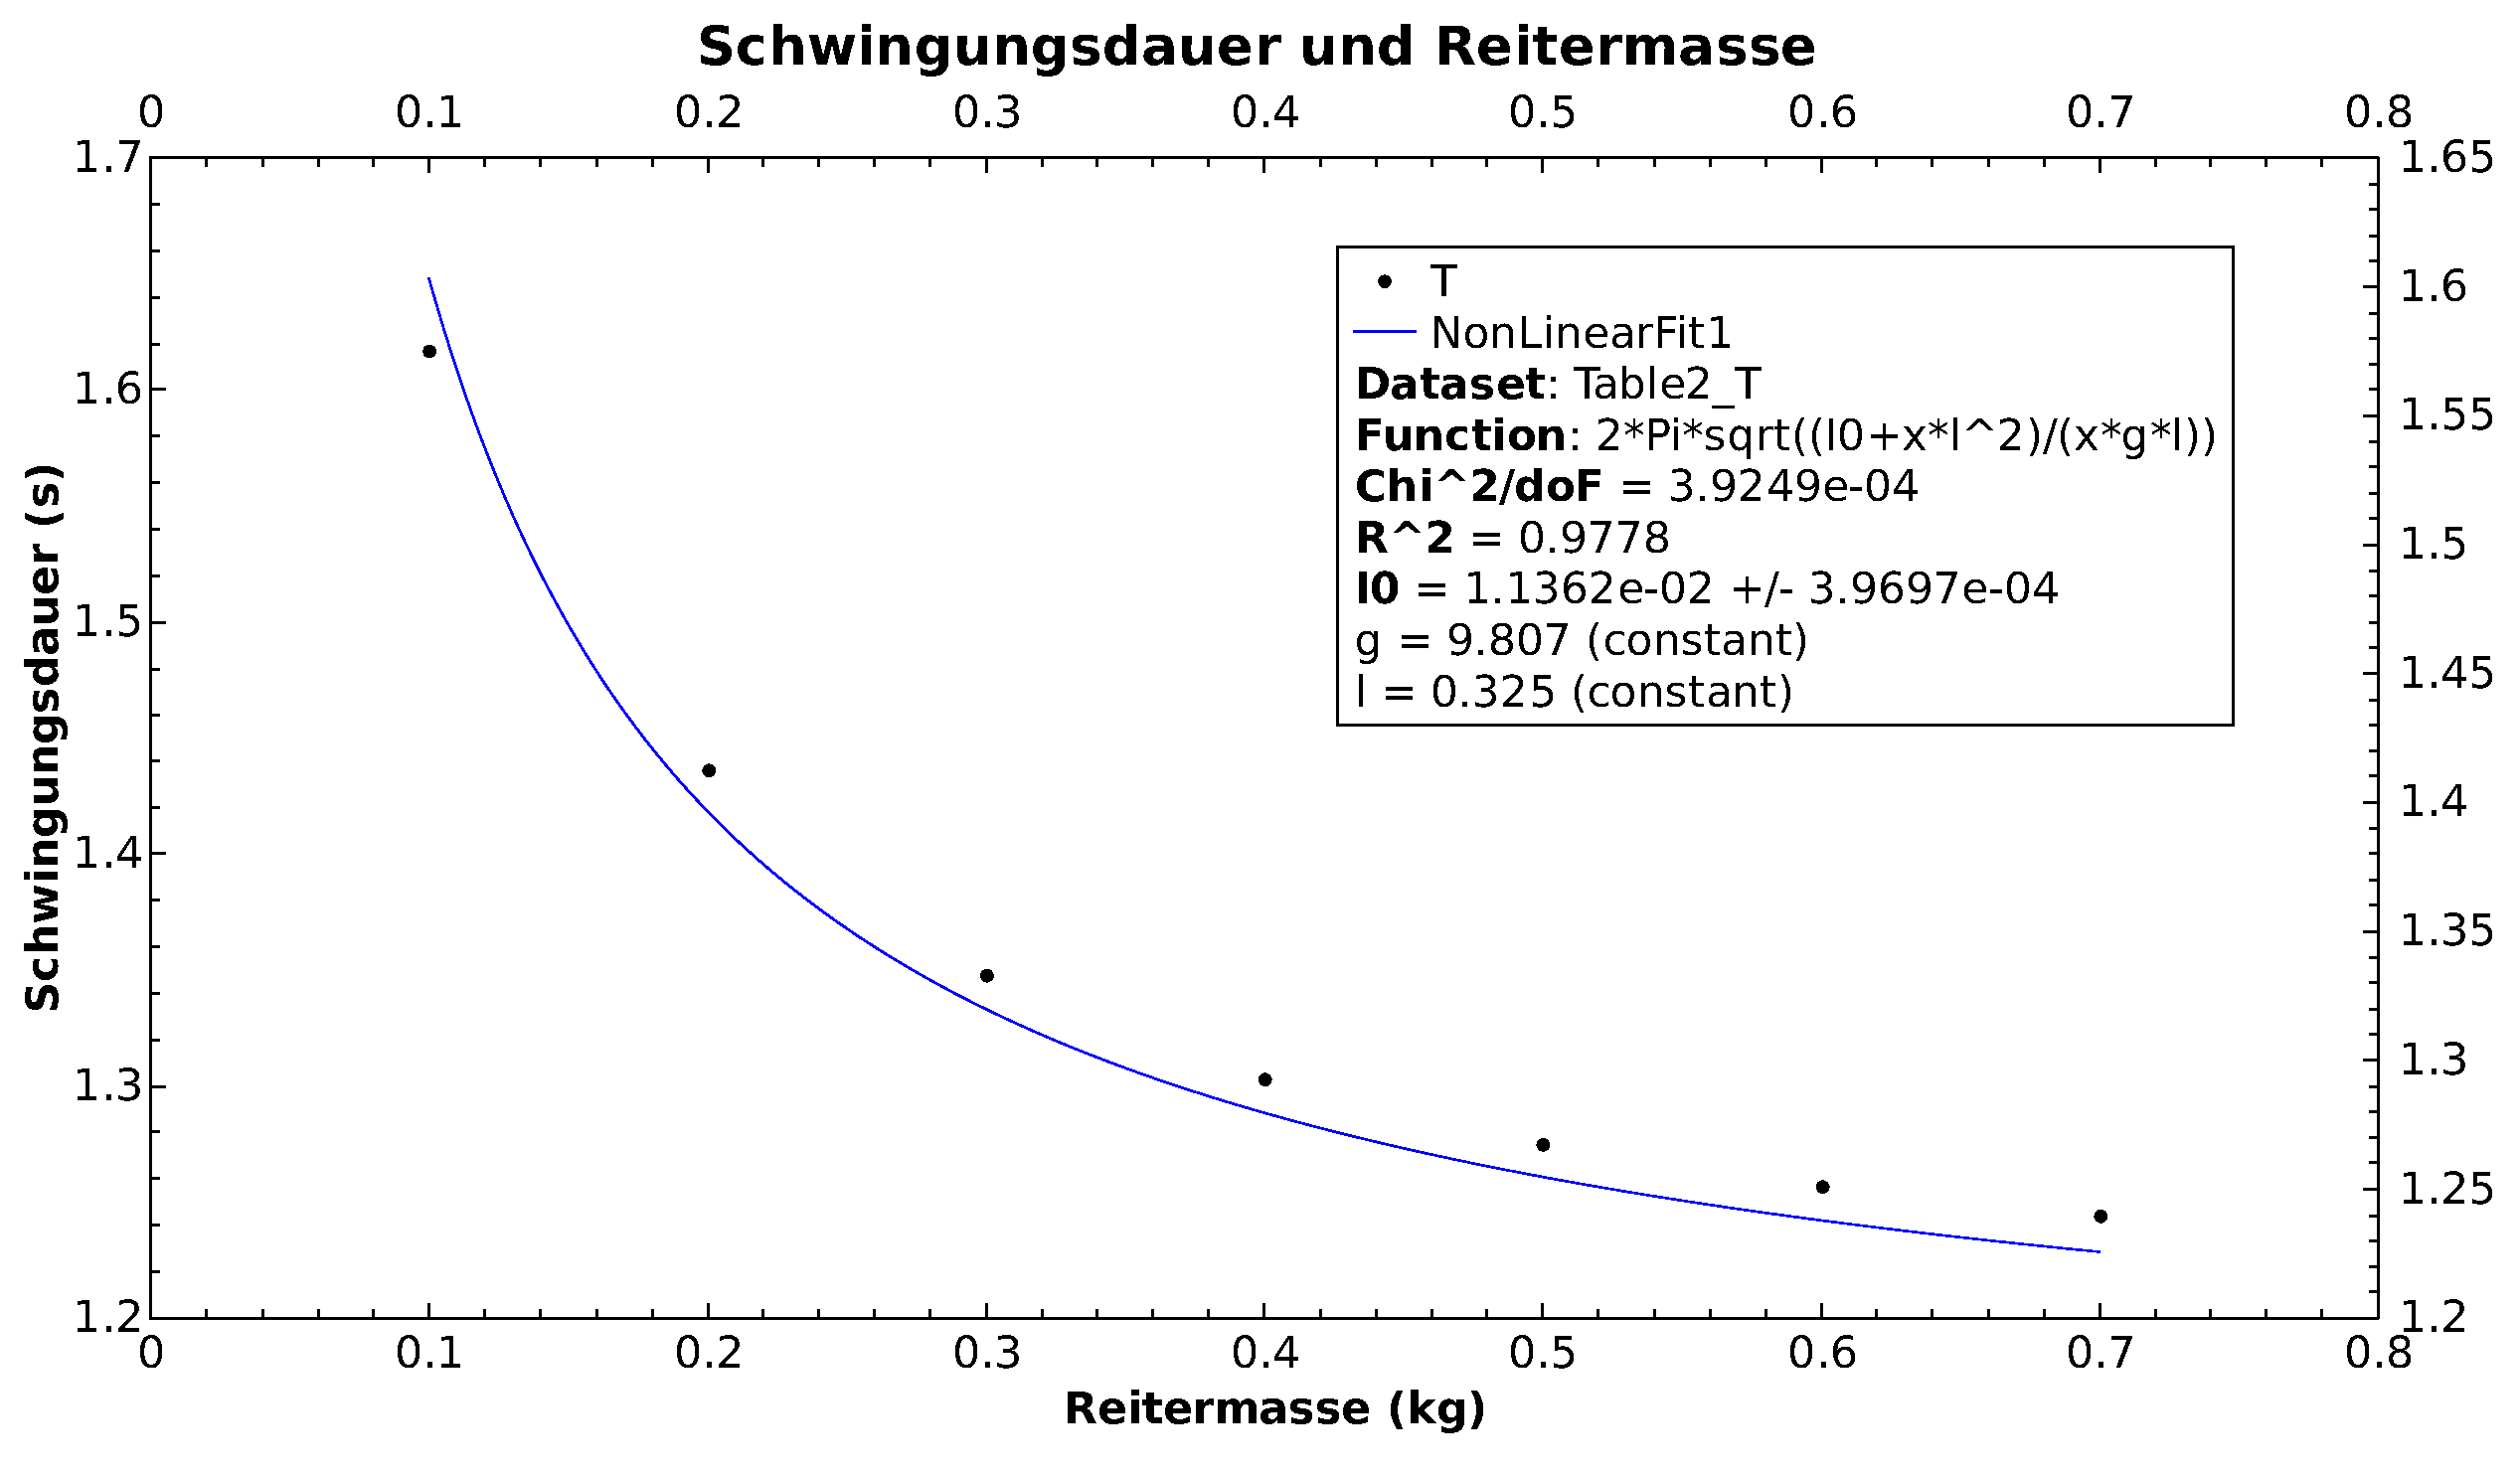
\includegraphics[width=\textwidth]{images/312.pdf}
    \caption{%
        Schwingungsdauer in Abh\"angigkeit der Reitermasse, gefitted \"uber Tr\"agheitsmoment. Abstand des Reiters war konstant \SI{325}{\milli\meter}.
    }
    \label{fig:312a}
\end{figure}

Wie man  in Abbildung  \ref{fig:312a} erkennen  kann, besteht  eine Abweichung
zwischen Fit  und Messwerten,  welche eine  zunehmende Tendenz  mit steigender
Reitermasse aufweist. Ich  f\"uhre das auf die  zunehmende Diskrepanz zwischen
der Ann\"aherung des Reiters als Punktmasse  mit $I_{Reiter} = m\cdot a^2$ und
der Modellierung als Zylinder inklusive Steiner-Anteil durch
$I_{Reiter} = \frac{m}{12}(3  \cdot r^2  + h^2) +  m \cdot a^2$.

Ber\"ucksichtigt  man die  Zylindrigkeit  des Reiters  und den  Steiner-Anteil
(siehe Abbildung \ref{fig:312b}), ergibt sich ein Massentr\"agheitsmoment von
$I_0  = \SI[separate-uncertainty = true]{11.297 \pm 0.36271}{\gram\meter\squared}$.

\begin{figure}[h!]
    \centering
    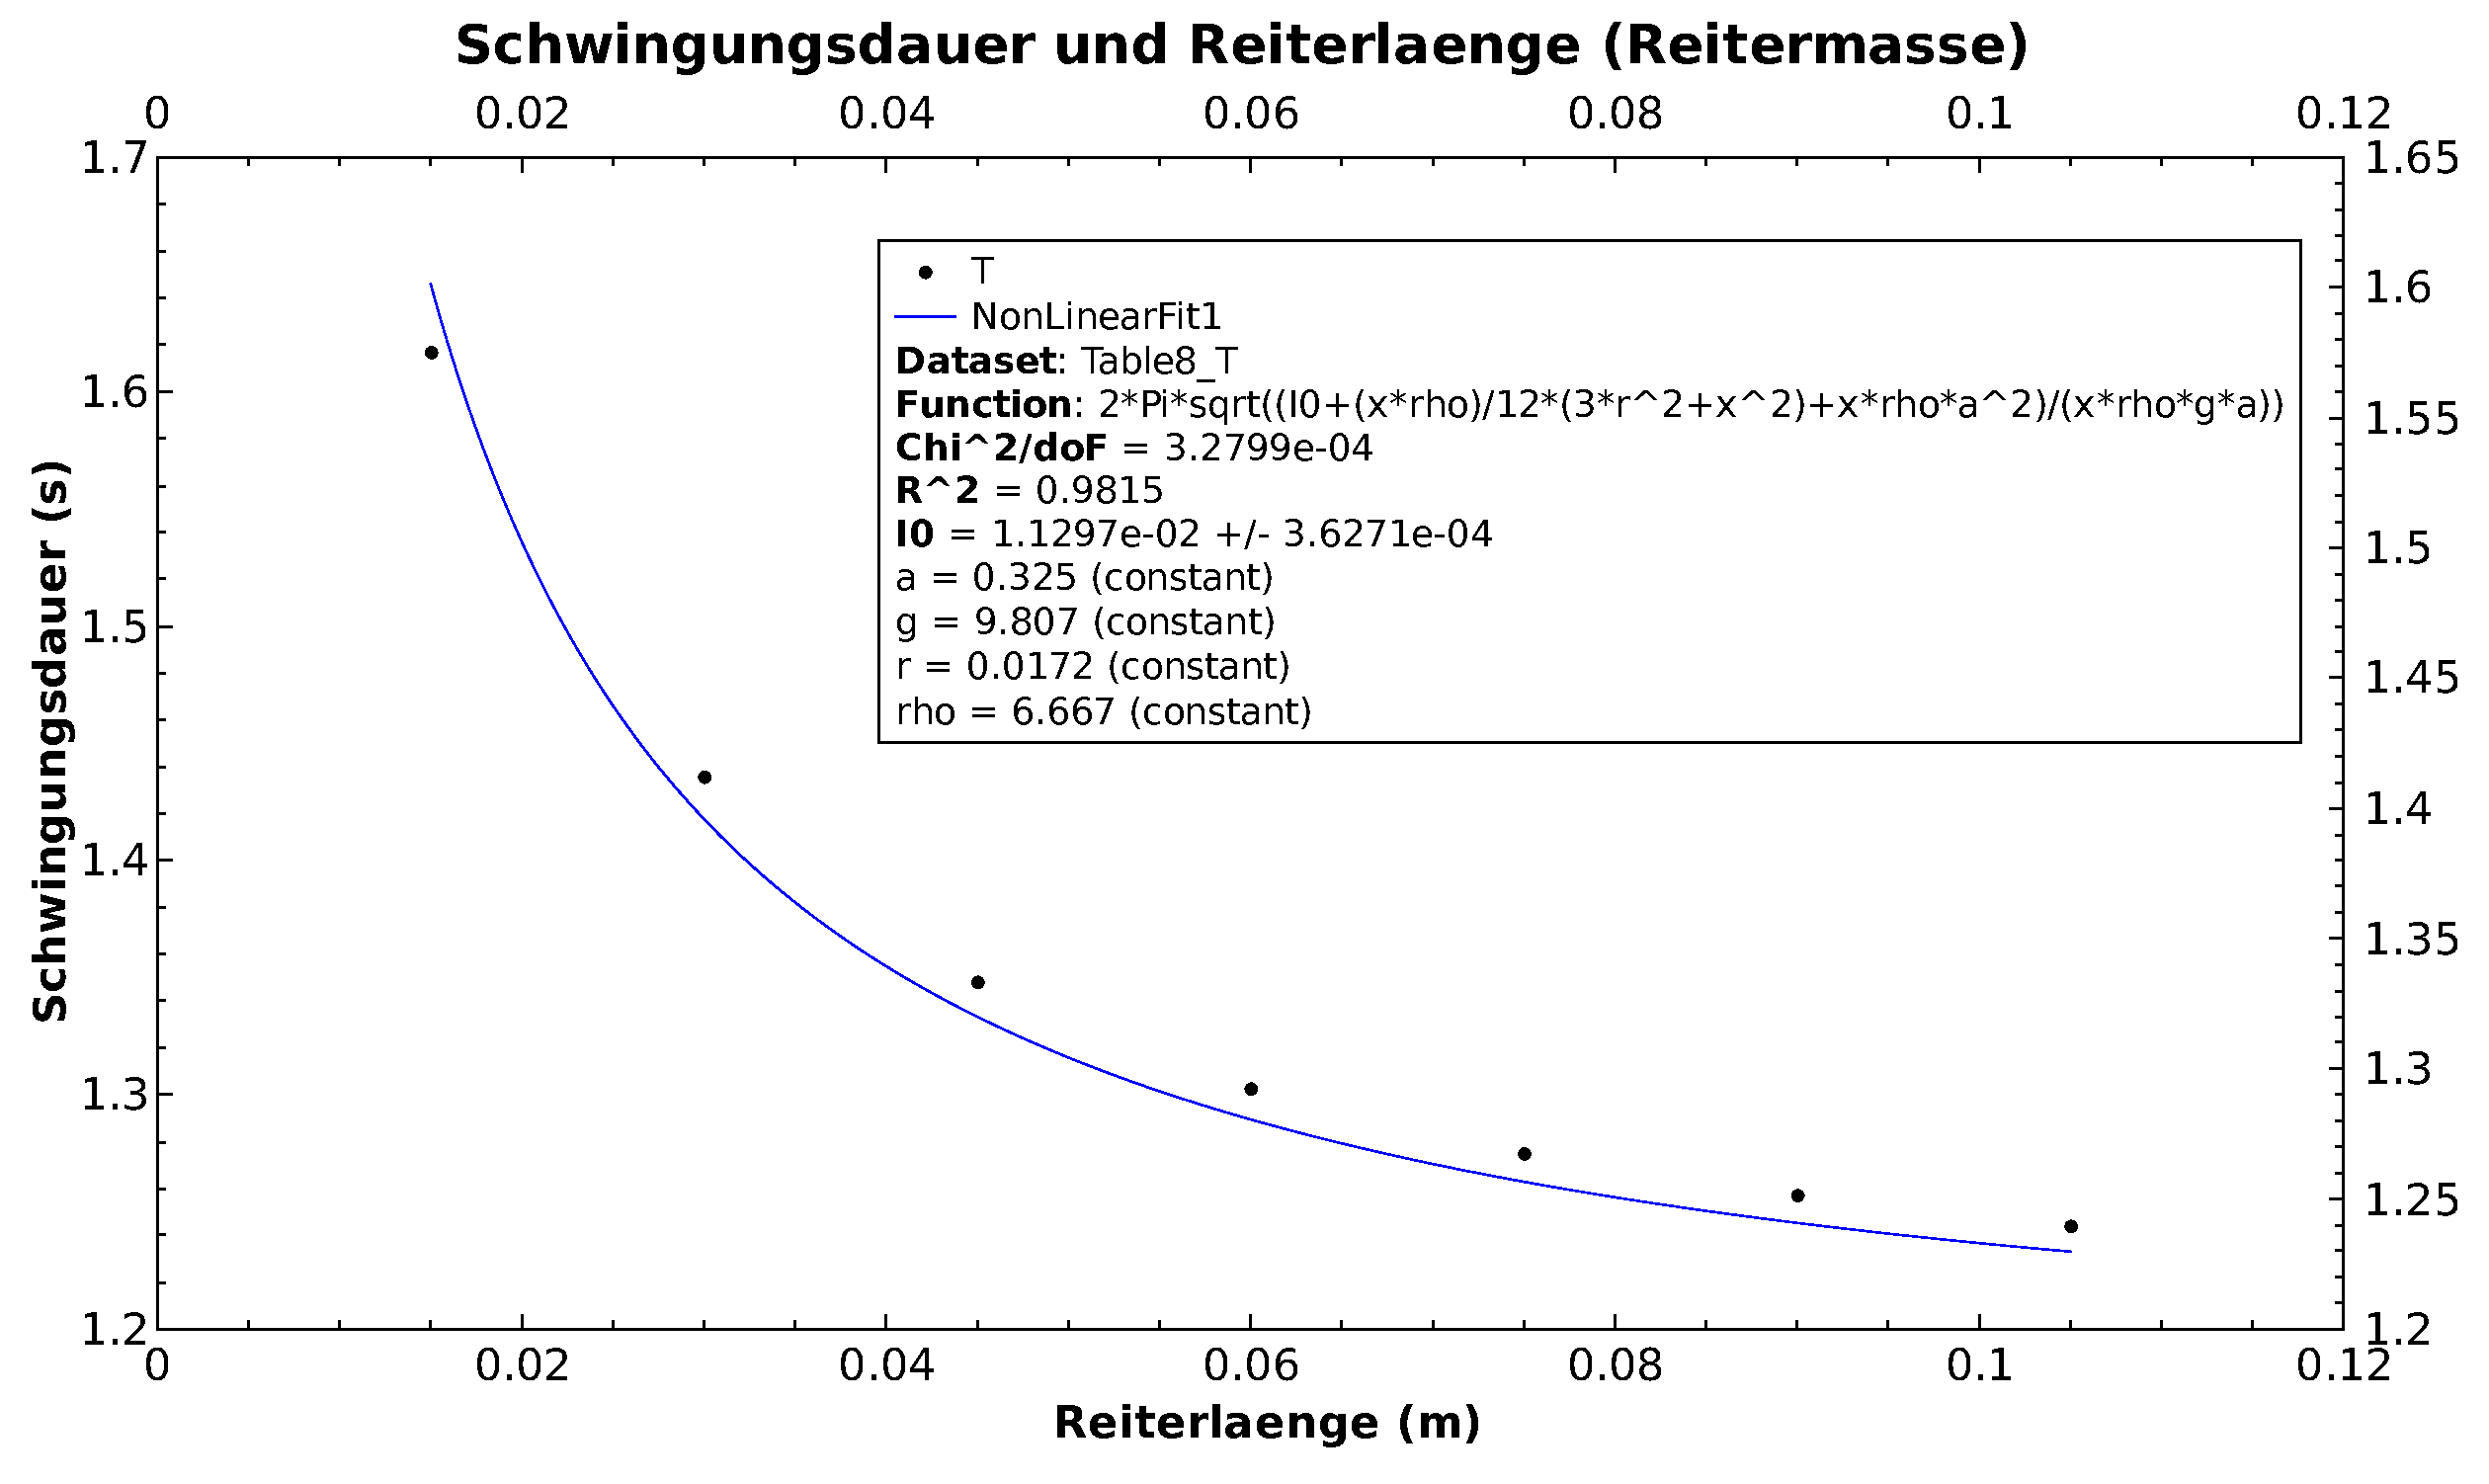
\includegraphics[width=\textwidth]{images/312b.pdf}
    \caption{%
        Schwingungsdauer in Abh\"angigkeit der Reitermasse, gefitted \"uber Tr\"agheitsmoment
    }
    \label{fig:312b}
\end{figure}

\clearpage
Man  kann  in  Abbildung  \ref{fig:312b}  erkennen, dass  nach  wie  vor  eine
Abweichung zwischen Fit und Messwerten besteht, allerdings scheint die Tendenz
der Differenz eher konstant und nicht zunehmend zu sein. Deshalb habe ich noch
einen  zus\"atzlichen  Fit  erstellt,  in dem  der  unterste  Messpunkt  nicht
ber\"ucksichtigt wird, was zum Fit in Abbildung \ref{fig:312c} f\"uhrt.

Dies ergibt
$I_0  = \SI[separate-uncertainty = true]{12.311 \pm 0.092950}{\gram\meter\squared}$.
Interessanterweise  ist die  Unsicherheit  hier merklich  kleiner, obwohl  ein
Messpunkt weniger verwendet wurde.

\begin{figure}[h!]
    \centering
    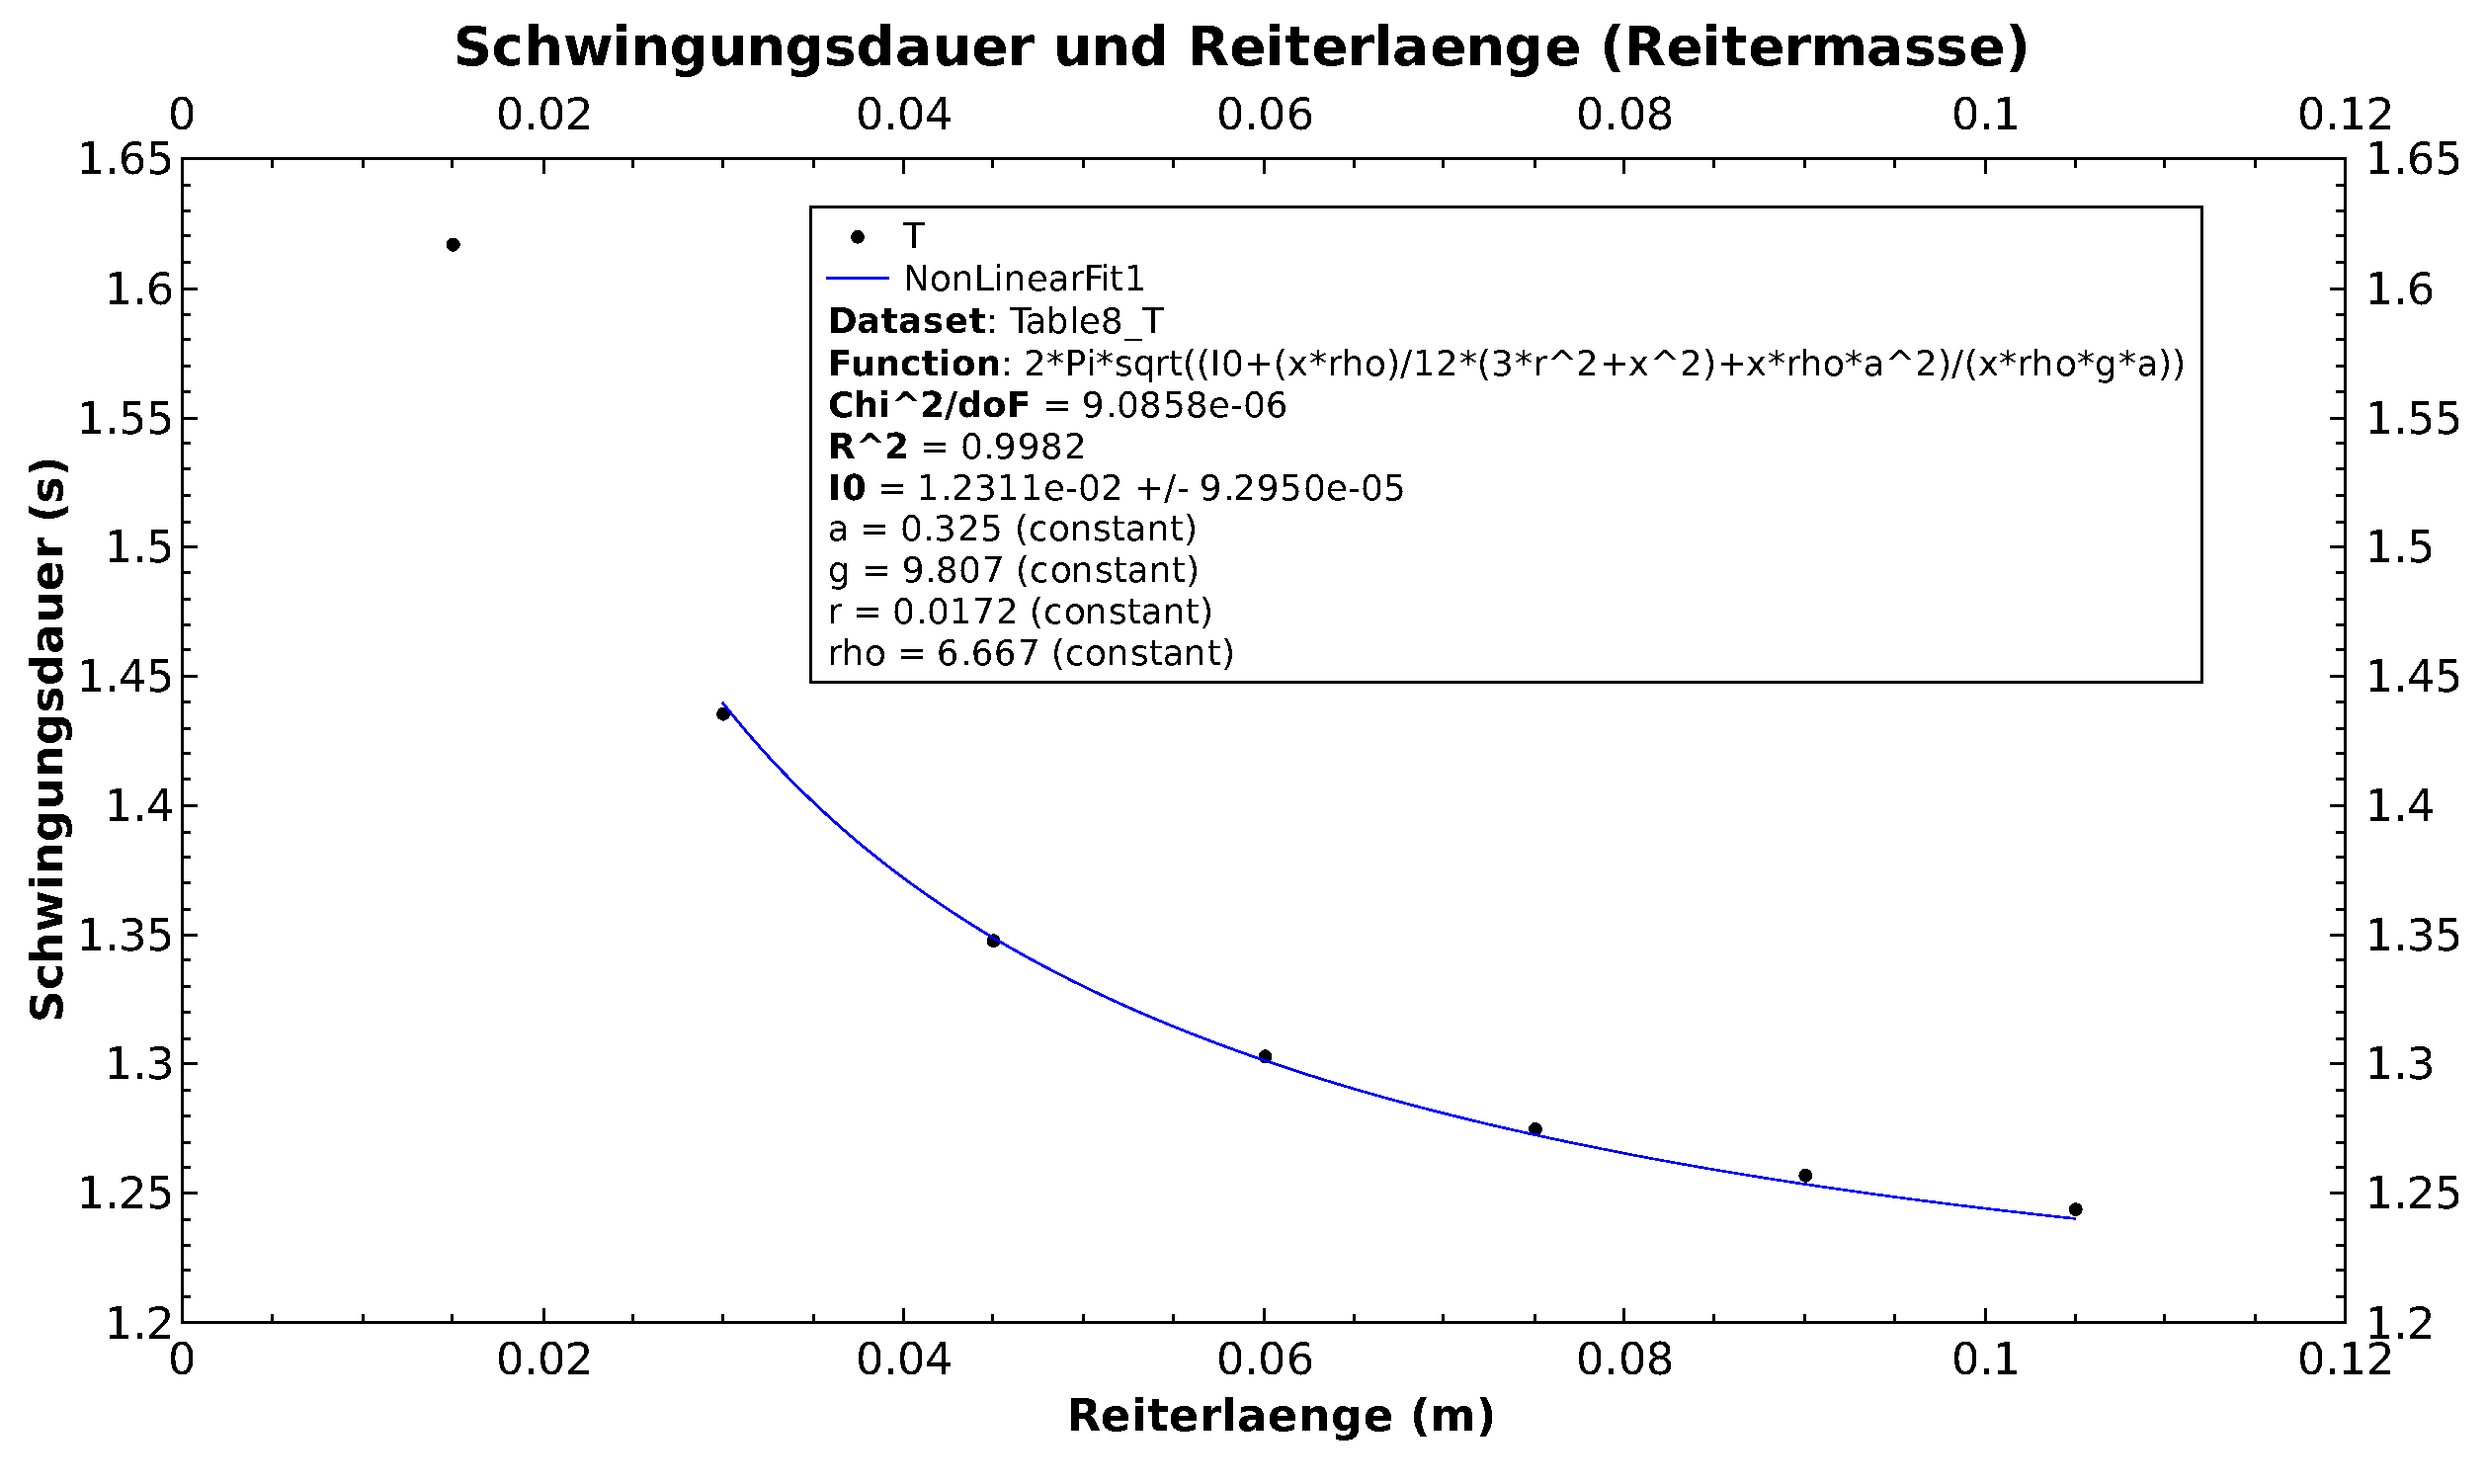
\includegraphics[width=\textwidth]{images/312c.pdf}
    \caption{%
        Schwingungsdauer in Abh\"angigkeit der Reitermasse, gefitted \"uber Tr\"agheitsmoment, unterster Messpunkt nicht ber\"ucksichtigt
    }
    \label{fig:312c}
\end{figure}

% ---------------------------------------------------------------------------- %
\clearpage
\subsection{Versuch 3.1.3 -- Periode in Abh\"angigkeit der Amplitude}
\label{subsec:periodeAmplitude}
% ---------------------------------------------------------------------------- %

Es wurde die gemessene Periode in Abh\"angigkeit der Amplitude mittels folgender
Formel gefittet:
\begin{equation}
    T = T_0 \cdot
        \left(
            1 +
            \left( \frac{1}{2} \right)^2 \cdot sin^2 \left( \frac{\hat{\varphi}}{2} \right)
            \left( \frac{1 \cdot 3}{2 \cdot 4} \right)^2 \cdot sin^4 \left( \frac{\hat{\varphi}}{2} \right)
            \left( \frac{1 \cdot 3 \cdot 5}{2 \cdot 4 \cdot 6} \right)^2 \cdot sin^6 \left( \frac{\hat{\varphi}}{2} \right)
            + ...
        \right)
\end{equation}

Zur Bestimmung der Anzahl n\"otigen Terme findet man im Anhang zu Versuch W4 folgendes
Diagramm:
\begin{figure}[h!]
    \centering
    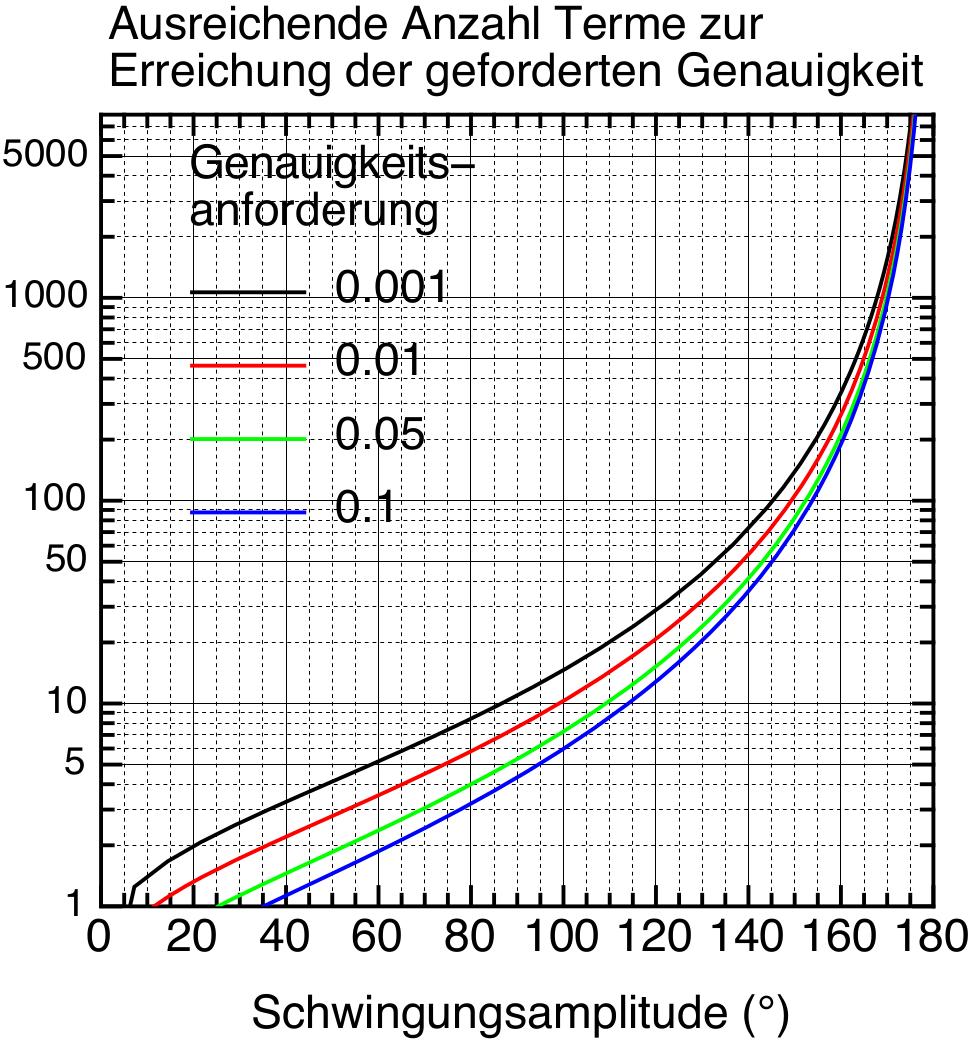
\includegraphics[width=.67\textwidth]{images/w4terme.png}
    \label{fig:w4terme}
    \caption{%
        Anzahl n\"otiger Terme in Abh\"angigkeit der gew\"unschten Genauigkeit
        und der maximalen Auslenkung.
    }
\end{figure}

Wir legen uns auf eine gew\"unschte Genauigkeit von \num{0.1} fest. Da wir bis
zu einem Winkel  von \SI{120}{\degree} gemessen haben,  ergibt dies ungef\"ahr
12 Terme (blaue Kurve).

Da  QtiPlot bei  12  Summanden abst\"urzte,  wurde die  Funktion  nur bis  zur
18. Potenz des Sinus gefittet.

\begin{figure}[h!]
    \centering
    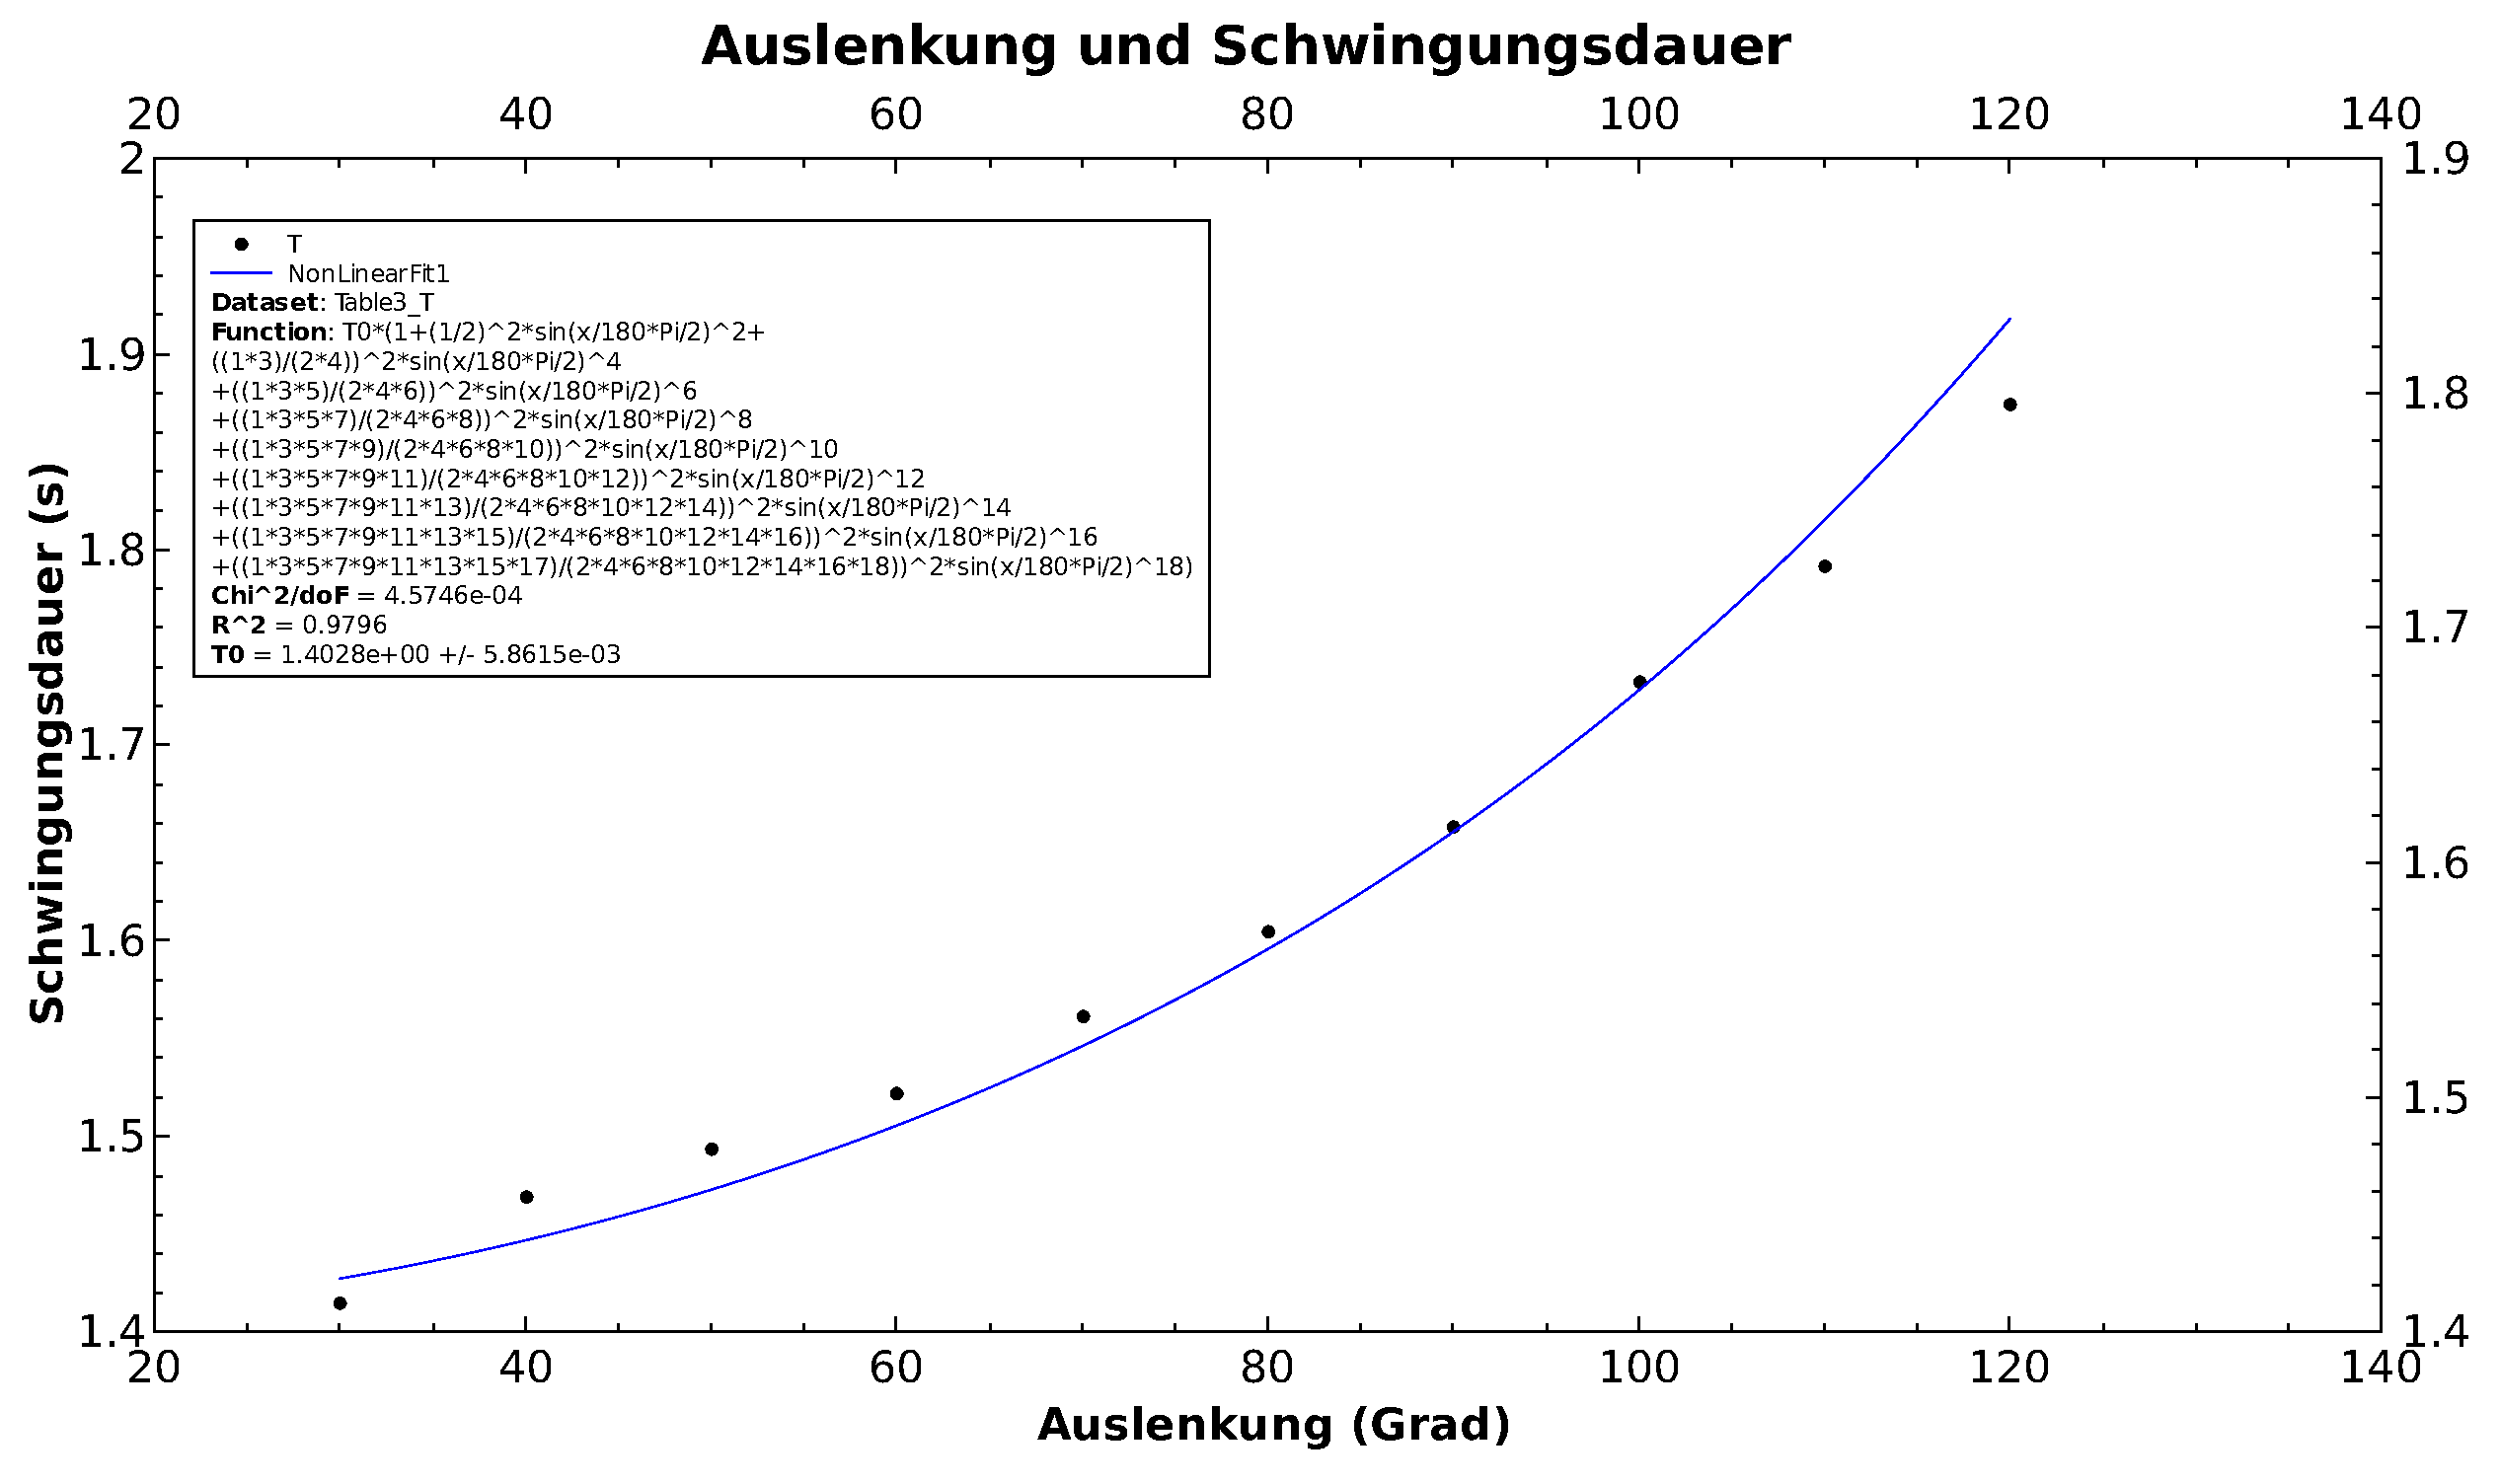
\includegraphics[width=\textwidth]{images/313.pdf}
    \label{fig:pendelKonfigs}
    \caption{%
        Schwingungsdauer in Abh\"angigkeit der Auslenkung
    }
\end{figure}

Da der  untereste Wert  nach einem  Ausreisser aussieht  und die  oberen Werte
aufgrund  von Reibungseffekten  vermutlich  nicht mehr  allzu pr\"azise  sind,
wurde noch ein zweiter Fit mit eingeschr\"anktem Bereich durchgef\"uhrt.

\begin{figure}[h!]
    \centering
    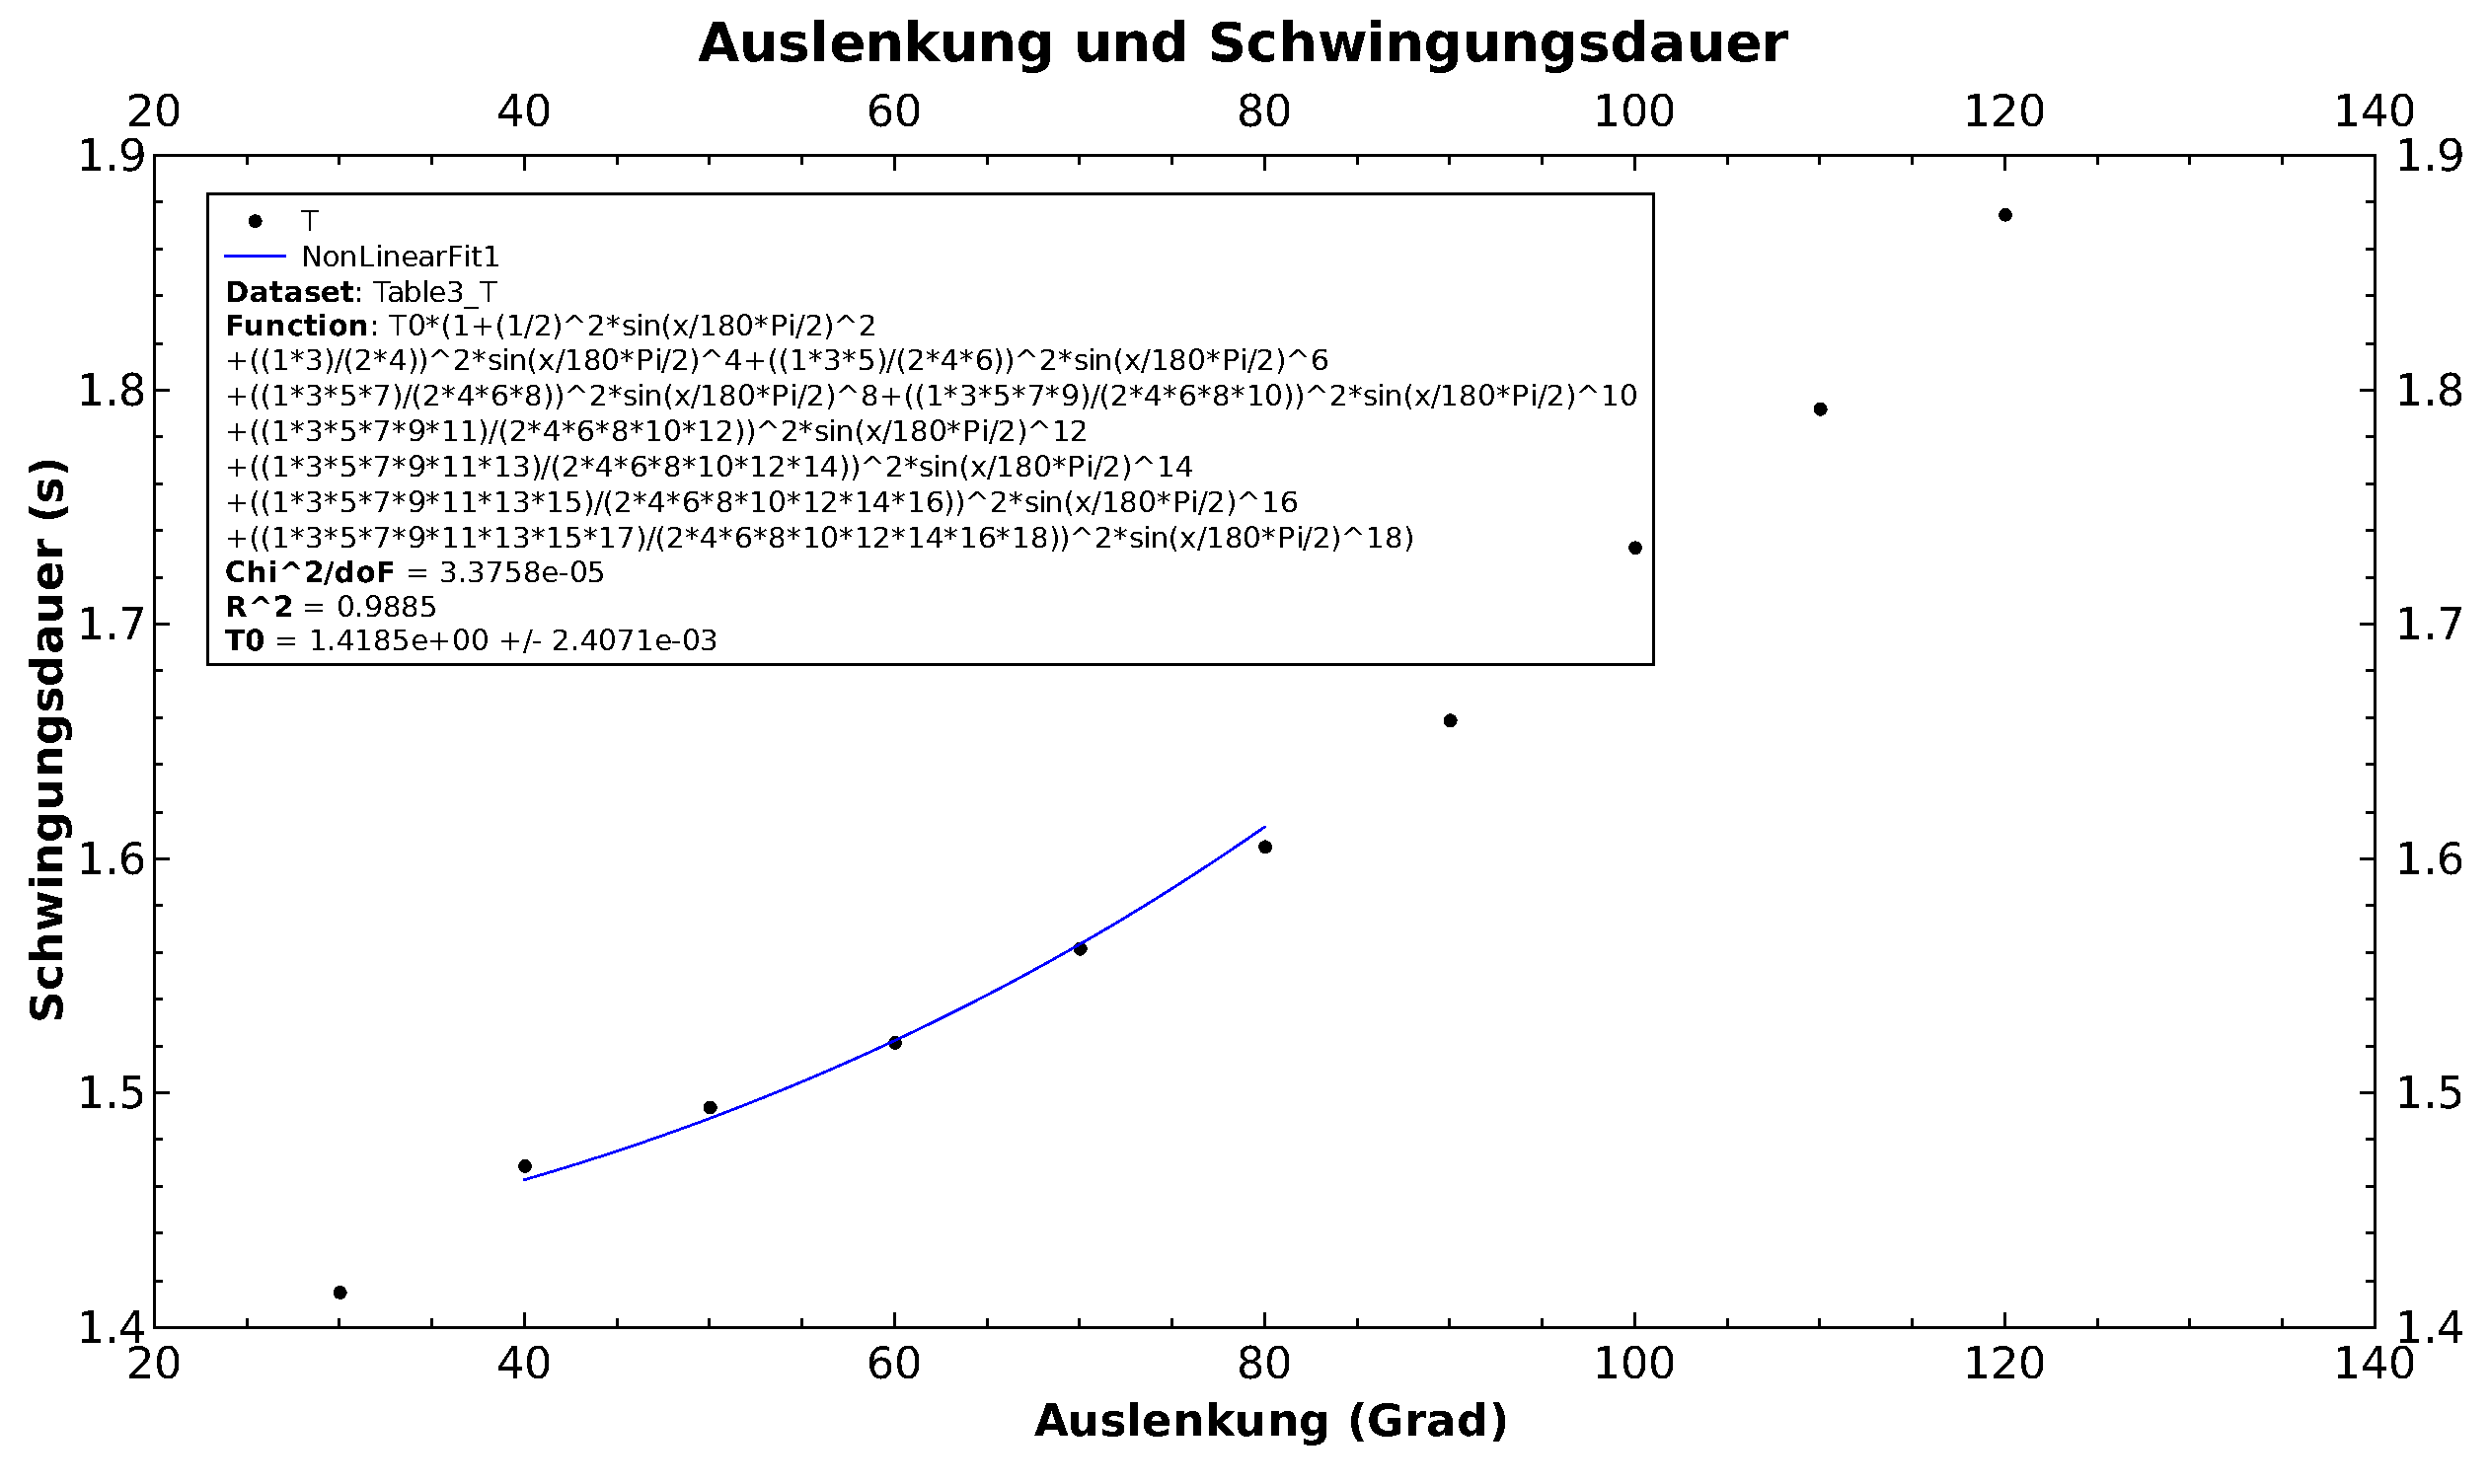
\includegraphics[width=\textwidth]{images/313b.pdf}
    \label{fig:pendelKonfigs}
    \caption{%
        Schwingungsdauer in Abh\"angigkeit der Auslenkung, eingeschr\"ankter Bereich.
    }
\end{figure}
$T_0  = \SI[separate-uncertainty = true]{1.4028 \pm 0.0058615}{\second}$.
$T_0  = \SI[separate-uncertainty = true]{1.4185 \pm 0.0024071}{\second}$.

% ---------------------------------------------------------------------------- %
\clearpage
\subsection{Versuch 3.3.1 -- Kombipendel Konfiguration 2}
\label{subsec:kombiKonfig2}
% ---------------------------------------------------------------------------- %


% ---------------------------------------------------------------------------- %
\subsubsection{Reiterposition variabel}
% ---------------------------------------------------------------------------- %

Hier wird folgende Formel zum Fitten verwendet:

\begin{equation}
    T = 2 \cdot \pi \cdot \sqrt{\frac{I}{p + q}}
\end{equation}

Die Federn und die Reitermasse wirken beide in die gleich Richtung r\"uckstellend,
daher das Plus-Zeichen im Nenner.

$I$ setzt sich  hier zusammen aus dem  oben bestimmten Massentr\"agheitsmoment
$I_0$ der Apparatur, aus  dem Massentr\"agheitsmoment $I_{Reiter}$ des Reiters
(approximiert  als   Punktmasse,  da  hier  der   Reiter  mit  \SI{200}{\gram}
verwendet  wurde)  und  dem  Anteil  $I_{Federn}$  der  Federn. Gefittet  wird
dann  \"uber die  Federkonstante $k$  im  Parameter $p  = 2kr^2$,  wobei $r  =
\SI{80.2}{\milli\meter}$ der Angriffsradius der  Federn an der Seilscheibe ist
(plus der Radius des Seils).

Es gilt also:
\begin{itemize}
    \item
        $I_0 = $
    \item
        $I_{Reiter} = \SI{200}{\gram} \cdot a^2$
    \item
        $I_{Federn} = \frac{1}{3} \cdot m_{Federn} \cdot \SI{80.2}{\milli\meter}^2$
    \item
        $p = 2 \cdot k \cdot \SI{80.2}{\milli\meter}^2$
    \item
        $q = m \cdot g \cdot a$ ($a$: Reiterposition)
\end{itemize}

Die   Masse   der   Federn    ist   \SI{155.5}{\gram}   f\"ur   beide   Federn
kombiniert. F\"ur das Massentr\"agheitsmoment $I_0$ verwenden wir den Wert von
\SI{12.311}{\gram\meter\squared} aus dem eingeschr\"ankten Fit.

Somit erh\"ahlt man als Formel f\"ur T:

\begin{equation}
    T = 2 \cdot \pi \cdot \sqrt{\frac{\SI{12.311}{\gram\meter\squared} + \SI{155.5}{\gram} \cdot (\SI{80.2}{\milli\meter})^2 + \SI{200}{\gram} \cdot a^2}{2 \cdot k \cdot (\SI{80.2}{\milli\meter})^2 + \SI{200}{\gram} \cdot
    \SI{9.807}{\meter\per\second\squared} \cdot a}}
\end{equation}

$a$ entspricht der x-Achse, gefittet wird \"uber $k$.

\begin{figure}[h!]
    \centering
    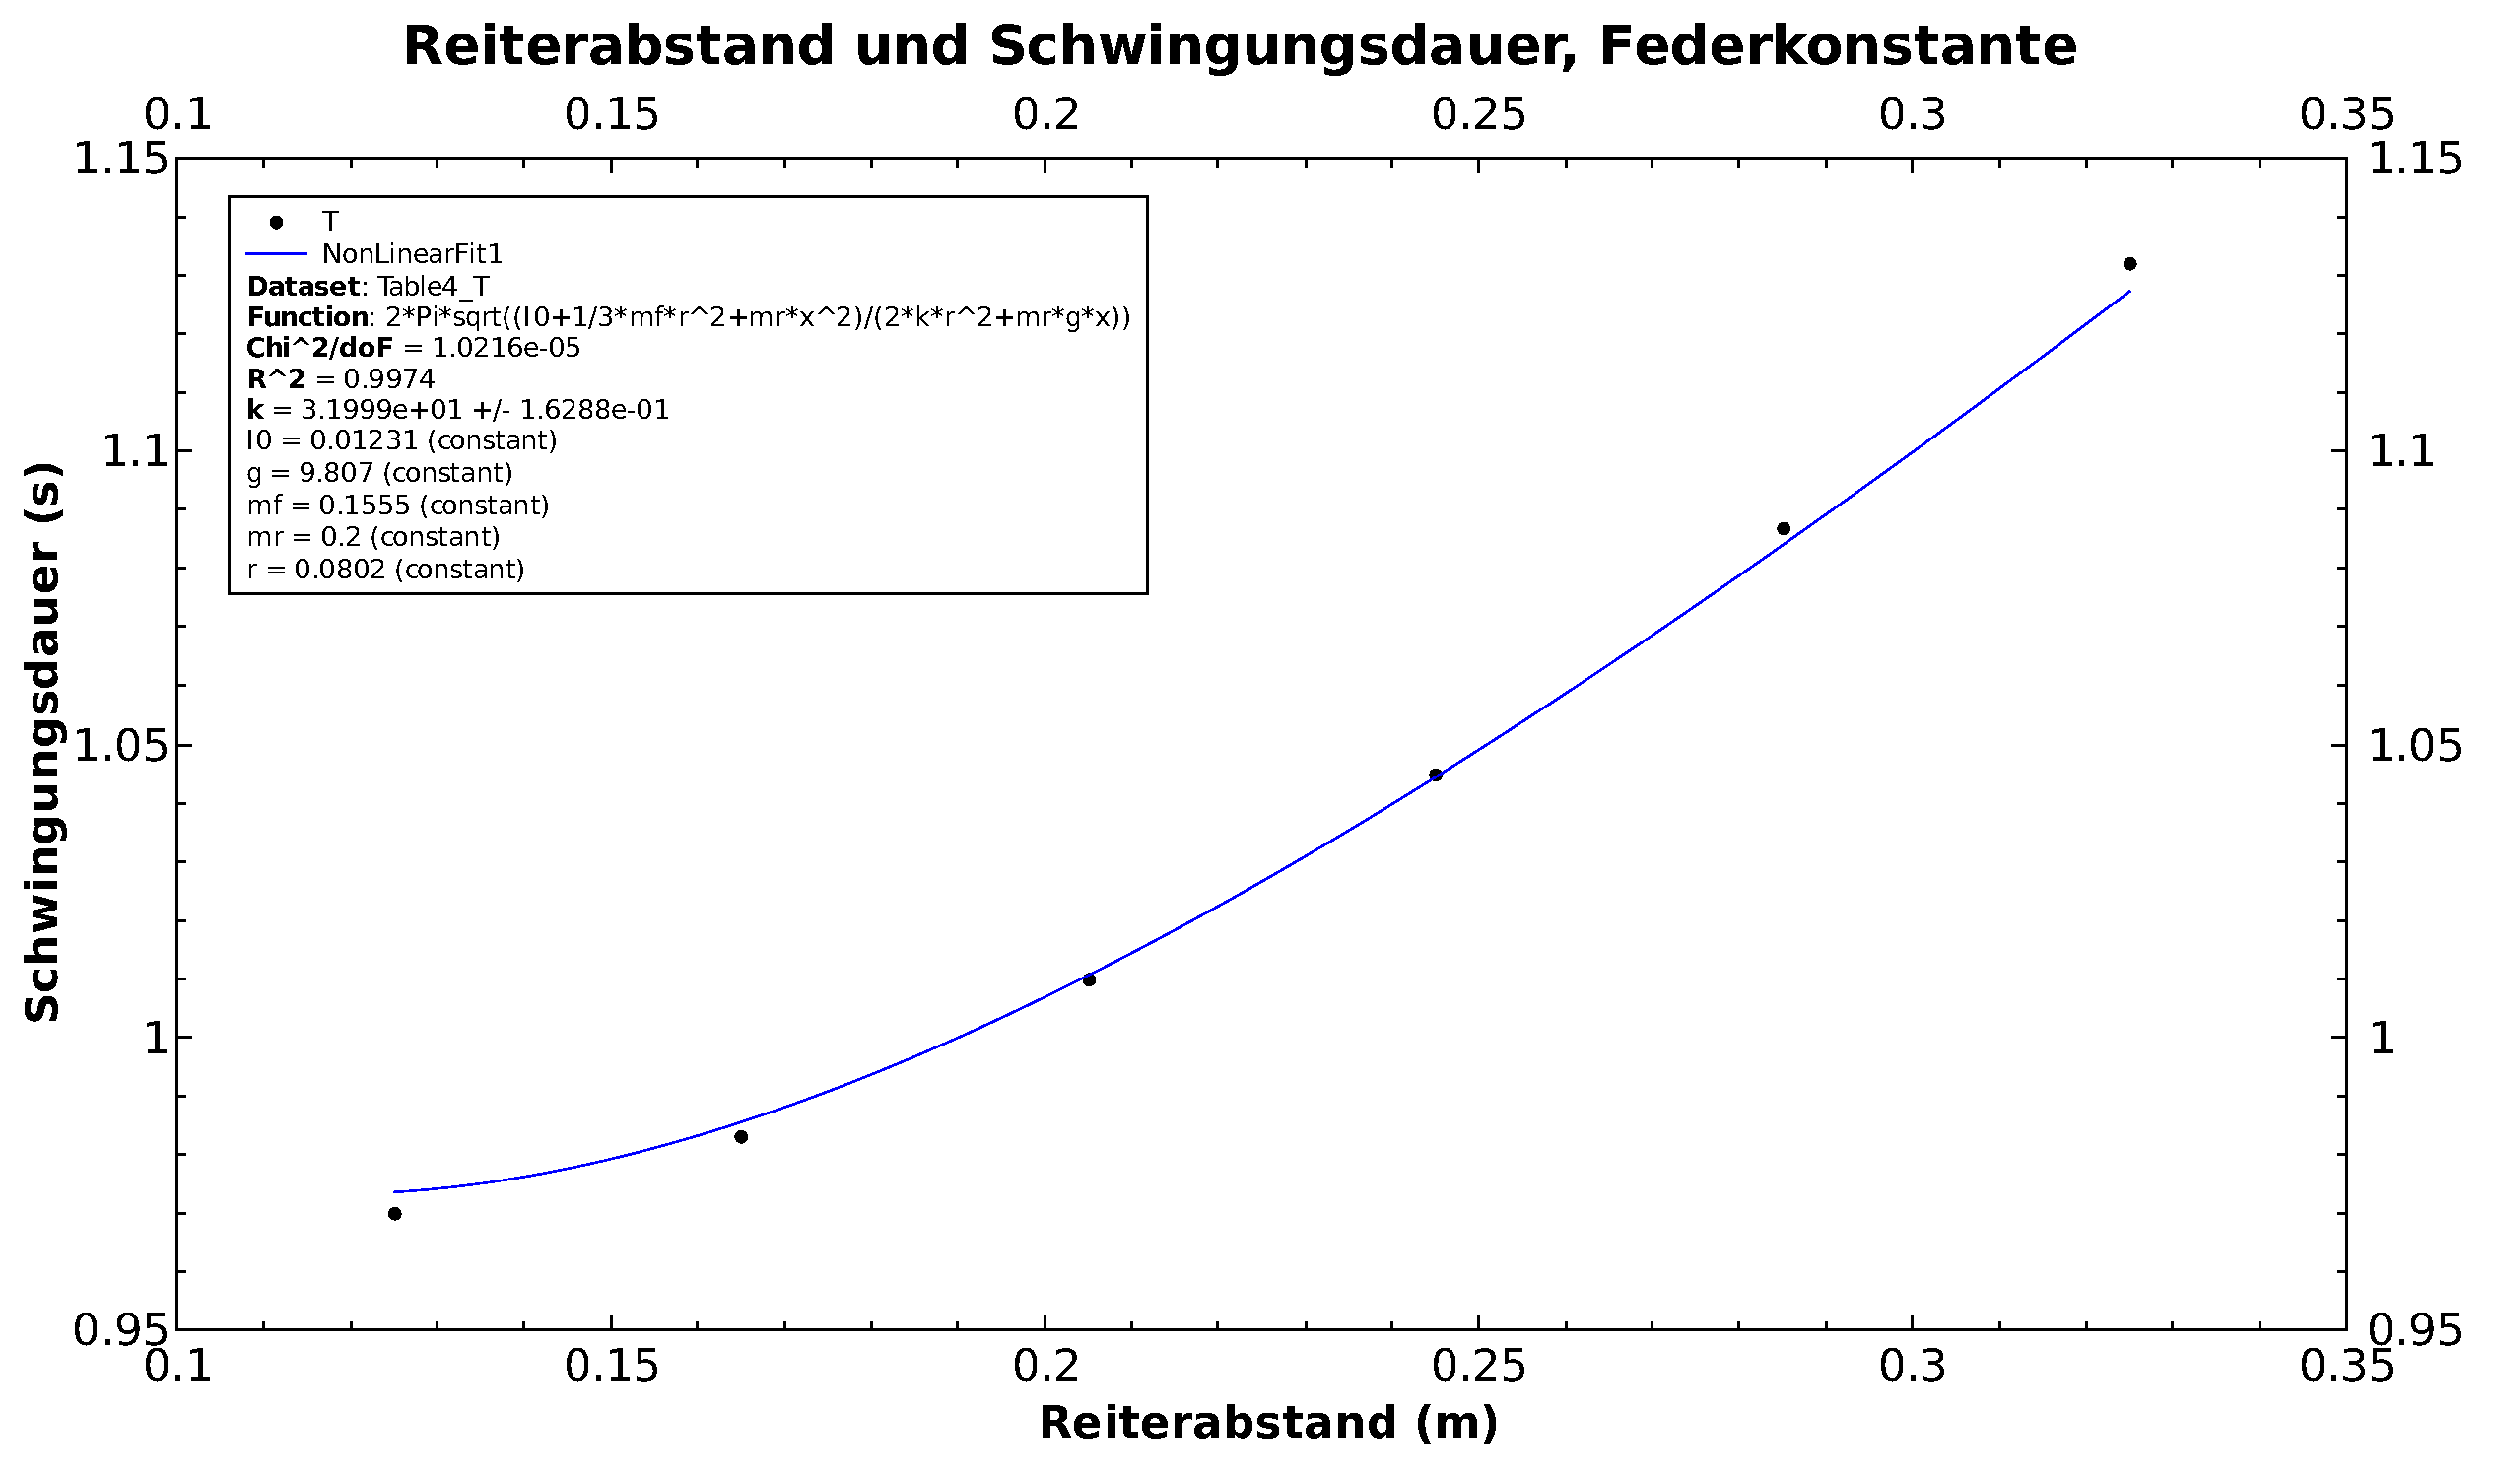
\includegraphics[width=\textwidth]{images/331a.pdf}
    \caption{%
        Schwingungsdauer in Abh\"angigkeit der Reiterposition beim Kombipendel, gefittet f\"ur Federkonstante $k$
    }
    \label{fig:331a}
\end{figure}

Aus dem  in Abbildung  \ref{fig:331a} dargestellten Fit  ergibt sich  ein Wert
f\"ur die  Federkonstante von  $k = \SI[separate-uncertainty  = true]{31.999
\pm  0.16288}{\newton\per\meter}$,  was  ziemlich   nahe  beim  Wert  aus  der
Versuchsanleitung von \SI{32}{\newton\per\meter} ist.


% ---------------------------------------------------------------------------- %
\clearpage
\subsubsection{Auslenkung variabel}
\label{subsubsec:kombiP:auslvar}
% ---------------------------------------------------------------------------- %

Bei dieser Messung stimmt offensichtlich etwas nicht so ganz, allerdings bin ich
mir nicht sicher, wo der Fehler genau liegt.


\begin{figure}[h!]
    \centering
    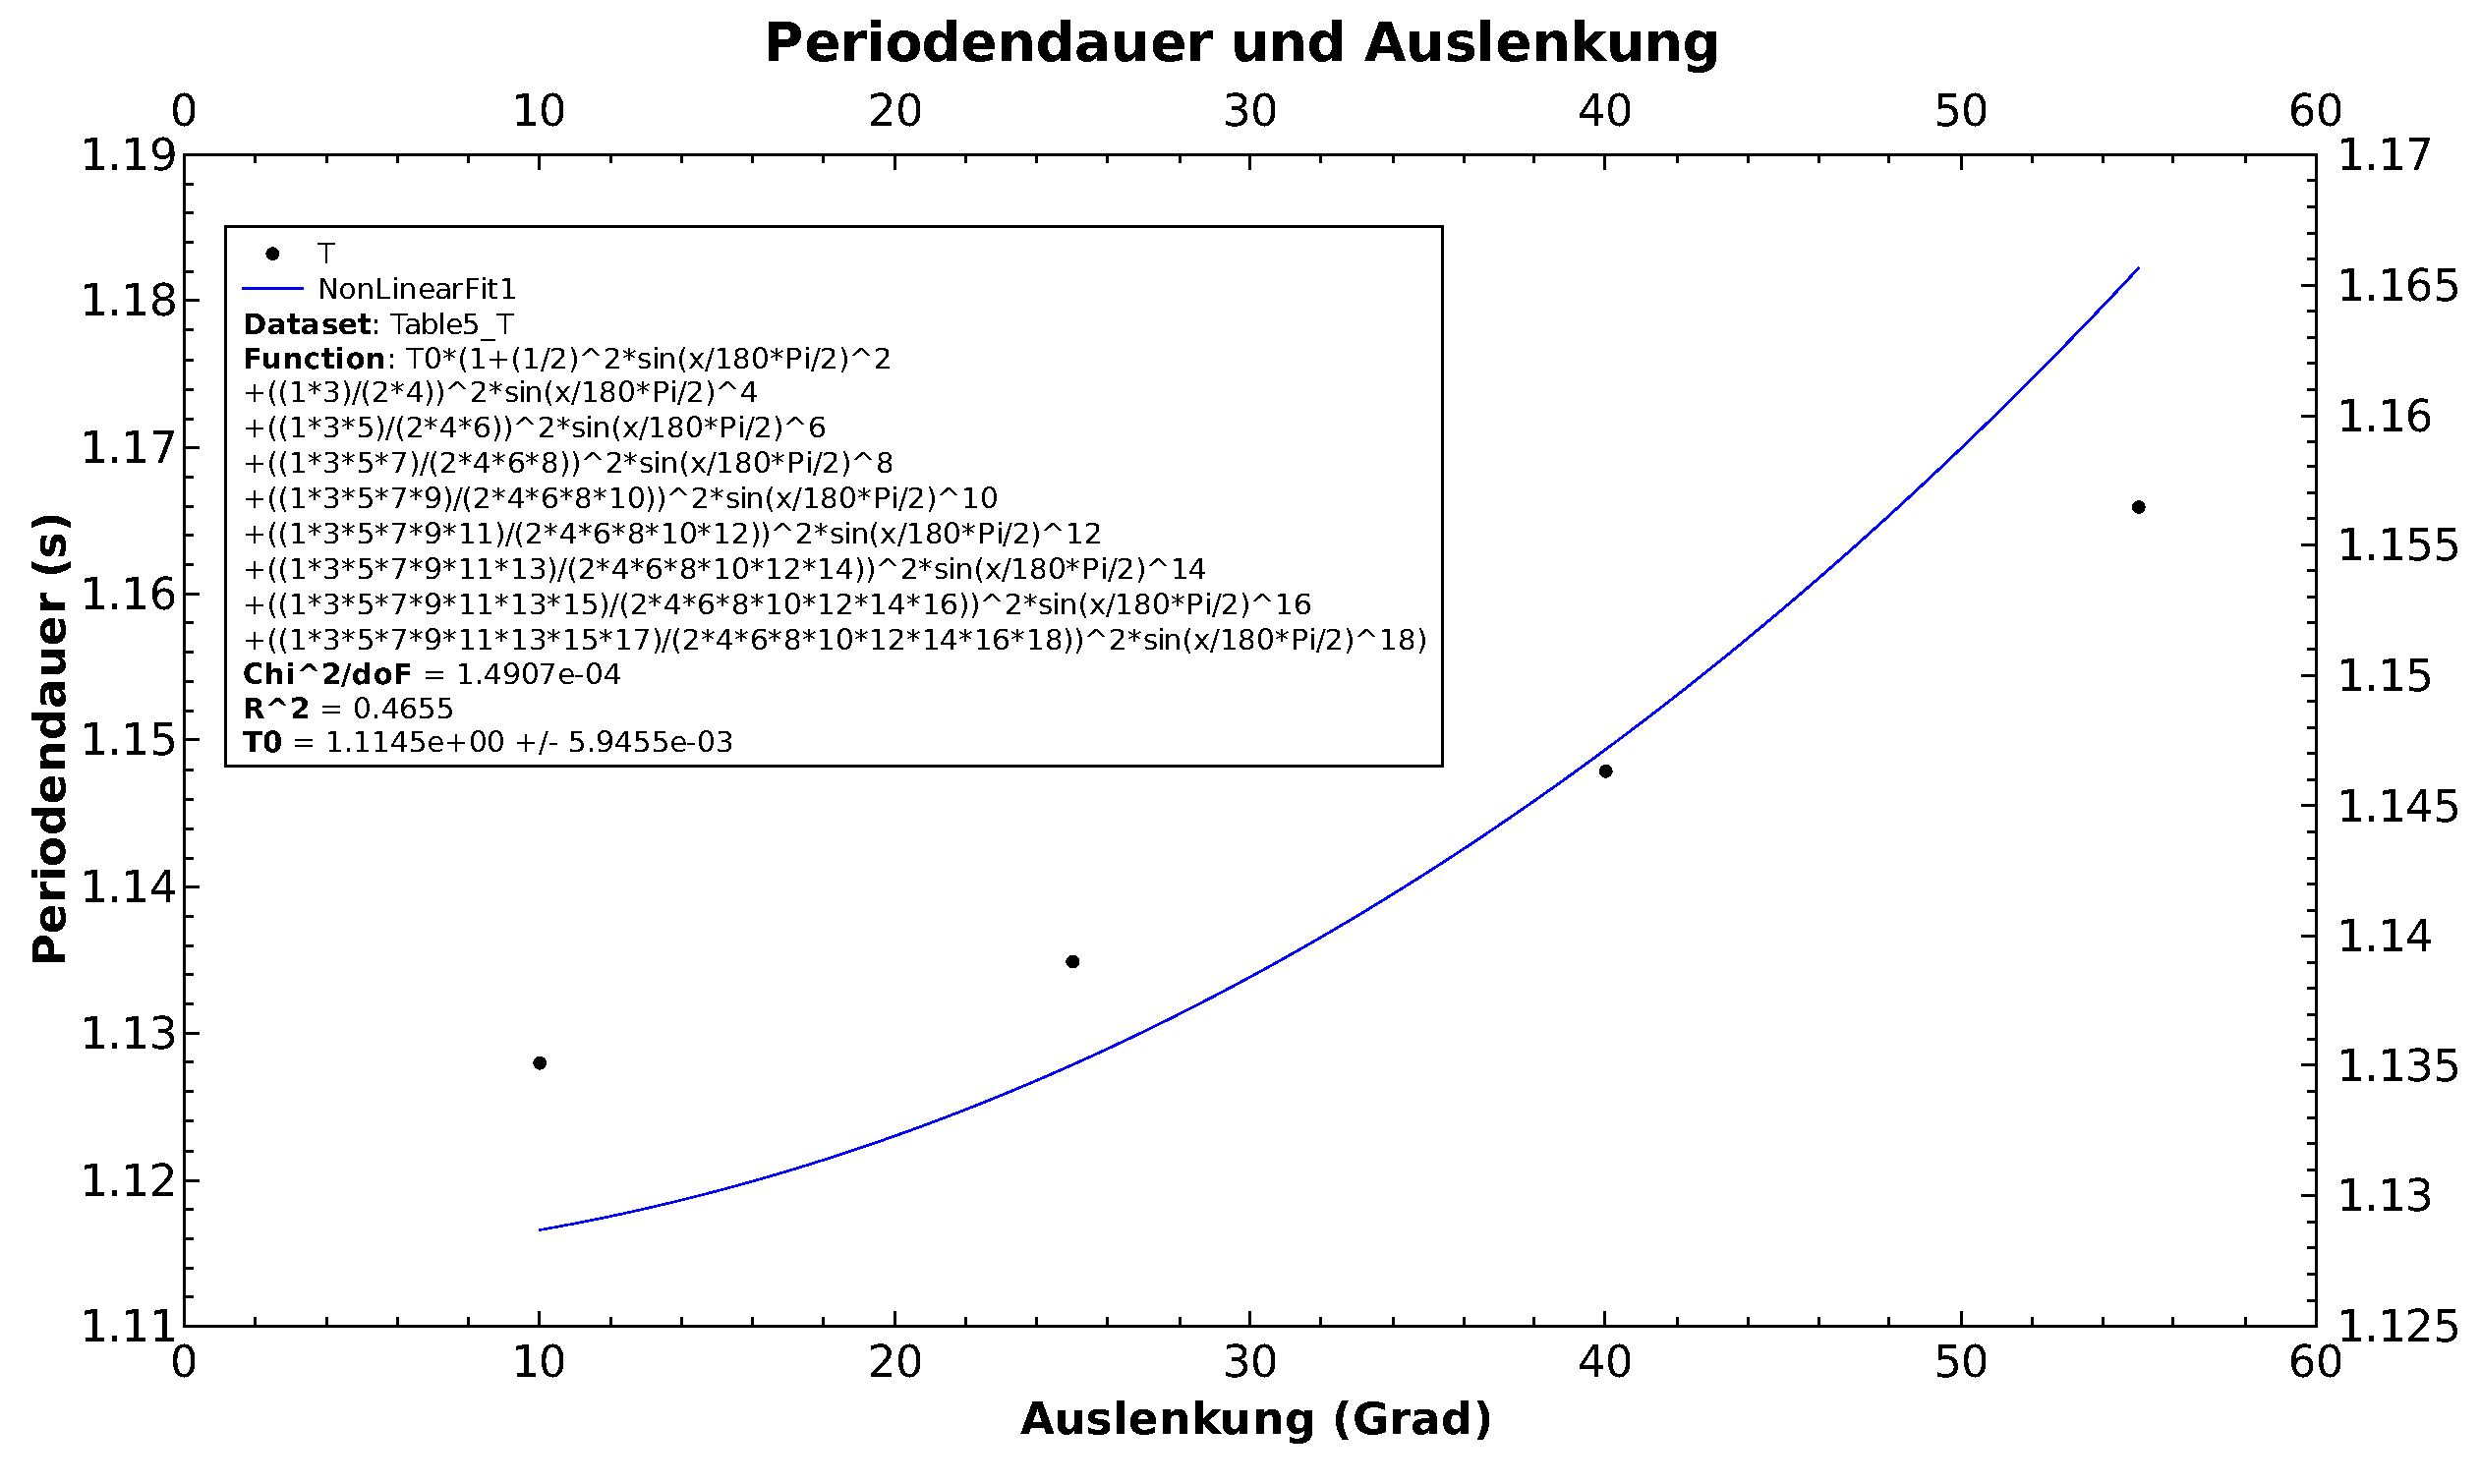
\includegraphics[width=\textwidth]{images/331b.pdf}
    \caption{%
        Schwingungsdauer in Abh\"angigkeit der Auslenkung beim Kombipendel
    }
    \label{fig:331b}
\end{figure}

Der   Fit   aus   Abbildung   \ref{fig:331b}  ergibt   einen   Wert   $T_0   =
\SI[separate-uncertainty  = true]{1.4028  \pm  0.0058615}{\second}$, was  zwar
einigermassen plausibel erscheint (verglichen  mit den Messwerten), jedoch ist
der Kurvenverlauf nicht wirklich passend zu den Messwerten. Allenfalls w\"aren
hier noch mehr Messungen durchzuf\"uhren.

F\"ur   die   Anzahl   Terme   wurden   hier   die   gleichen   \"Uberlegungen
gemacht  wie  bereits  in Abschnitt  \ref{subsec:periodeAmplitude}  auf  Seite
\pageref{subsec:periodeAmplitude} dokumentiert.




% ---------------------------------------------------------------------------- %
\clearpage
\subsection{Versuch 3.3.2 -- Kombipendel Konfiguration 3}
\label{subsec:kombiKonfig3}
% ---------------------------------------------------------------------------- %

Der  kritische  Abstand  $a_{krit}$  wurde  durch  Probieren  auf  einen  Wert
zwischen  $\SI{195}{\milli\meter}$ und  $\SI{205}{\milli\meter}$ bestimmt. Die
Versuchsreihe  wurde  daher mit  Werten  von  $a \leq  \SI{195}{\milli\meter}$
durchgef\"uhrt. Da Reitermasse und Federkraft sich hier entgegenwirken, ist im
Nenner zwischen $p$ und $q$ ein Minuszeichen zu finden.

\begin{figure}[h!]
    \centering
    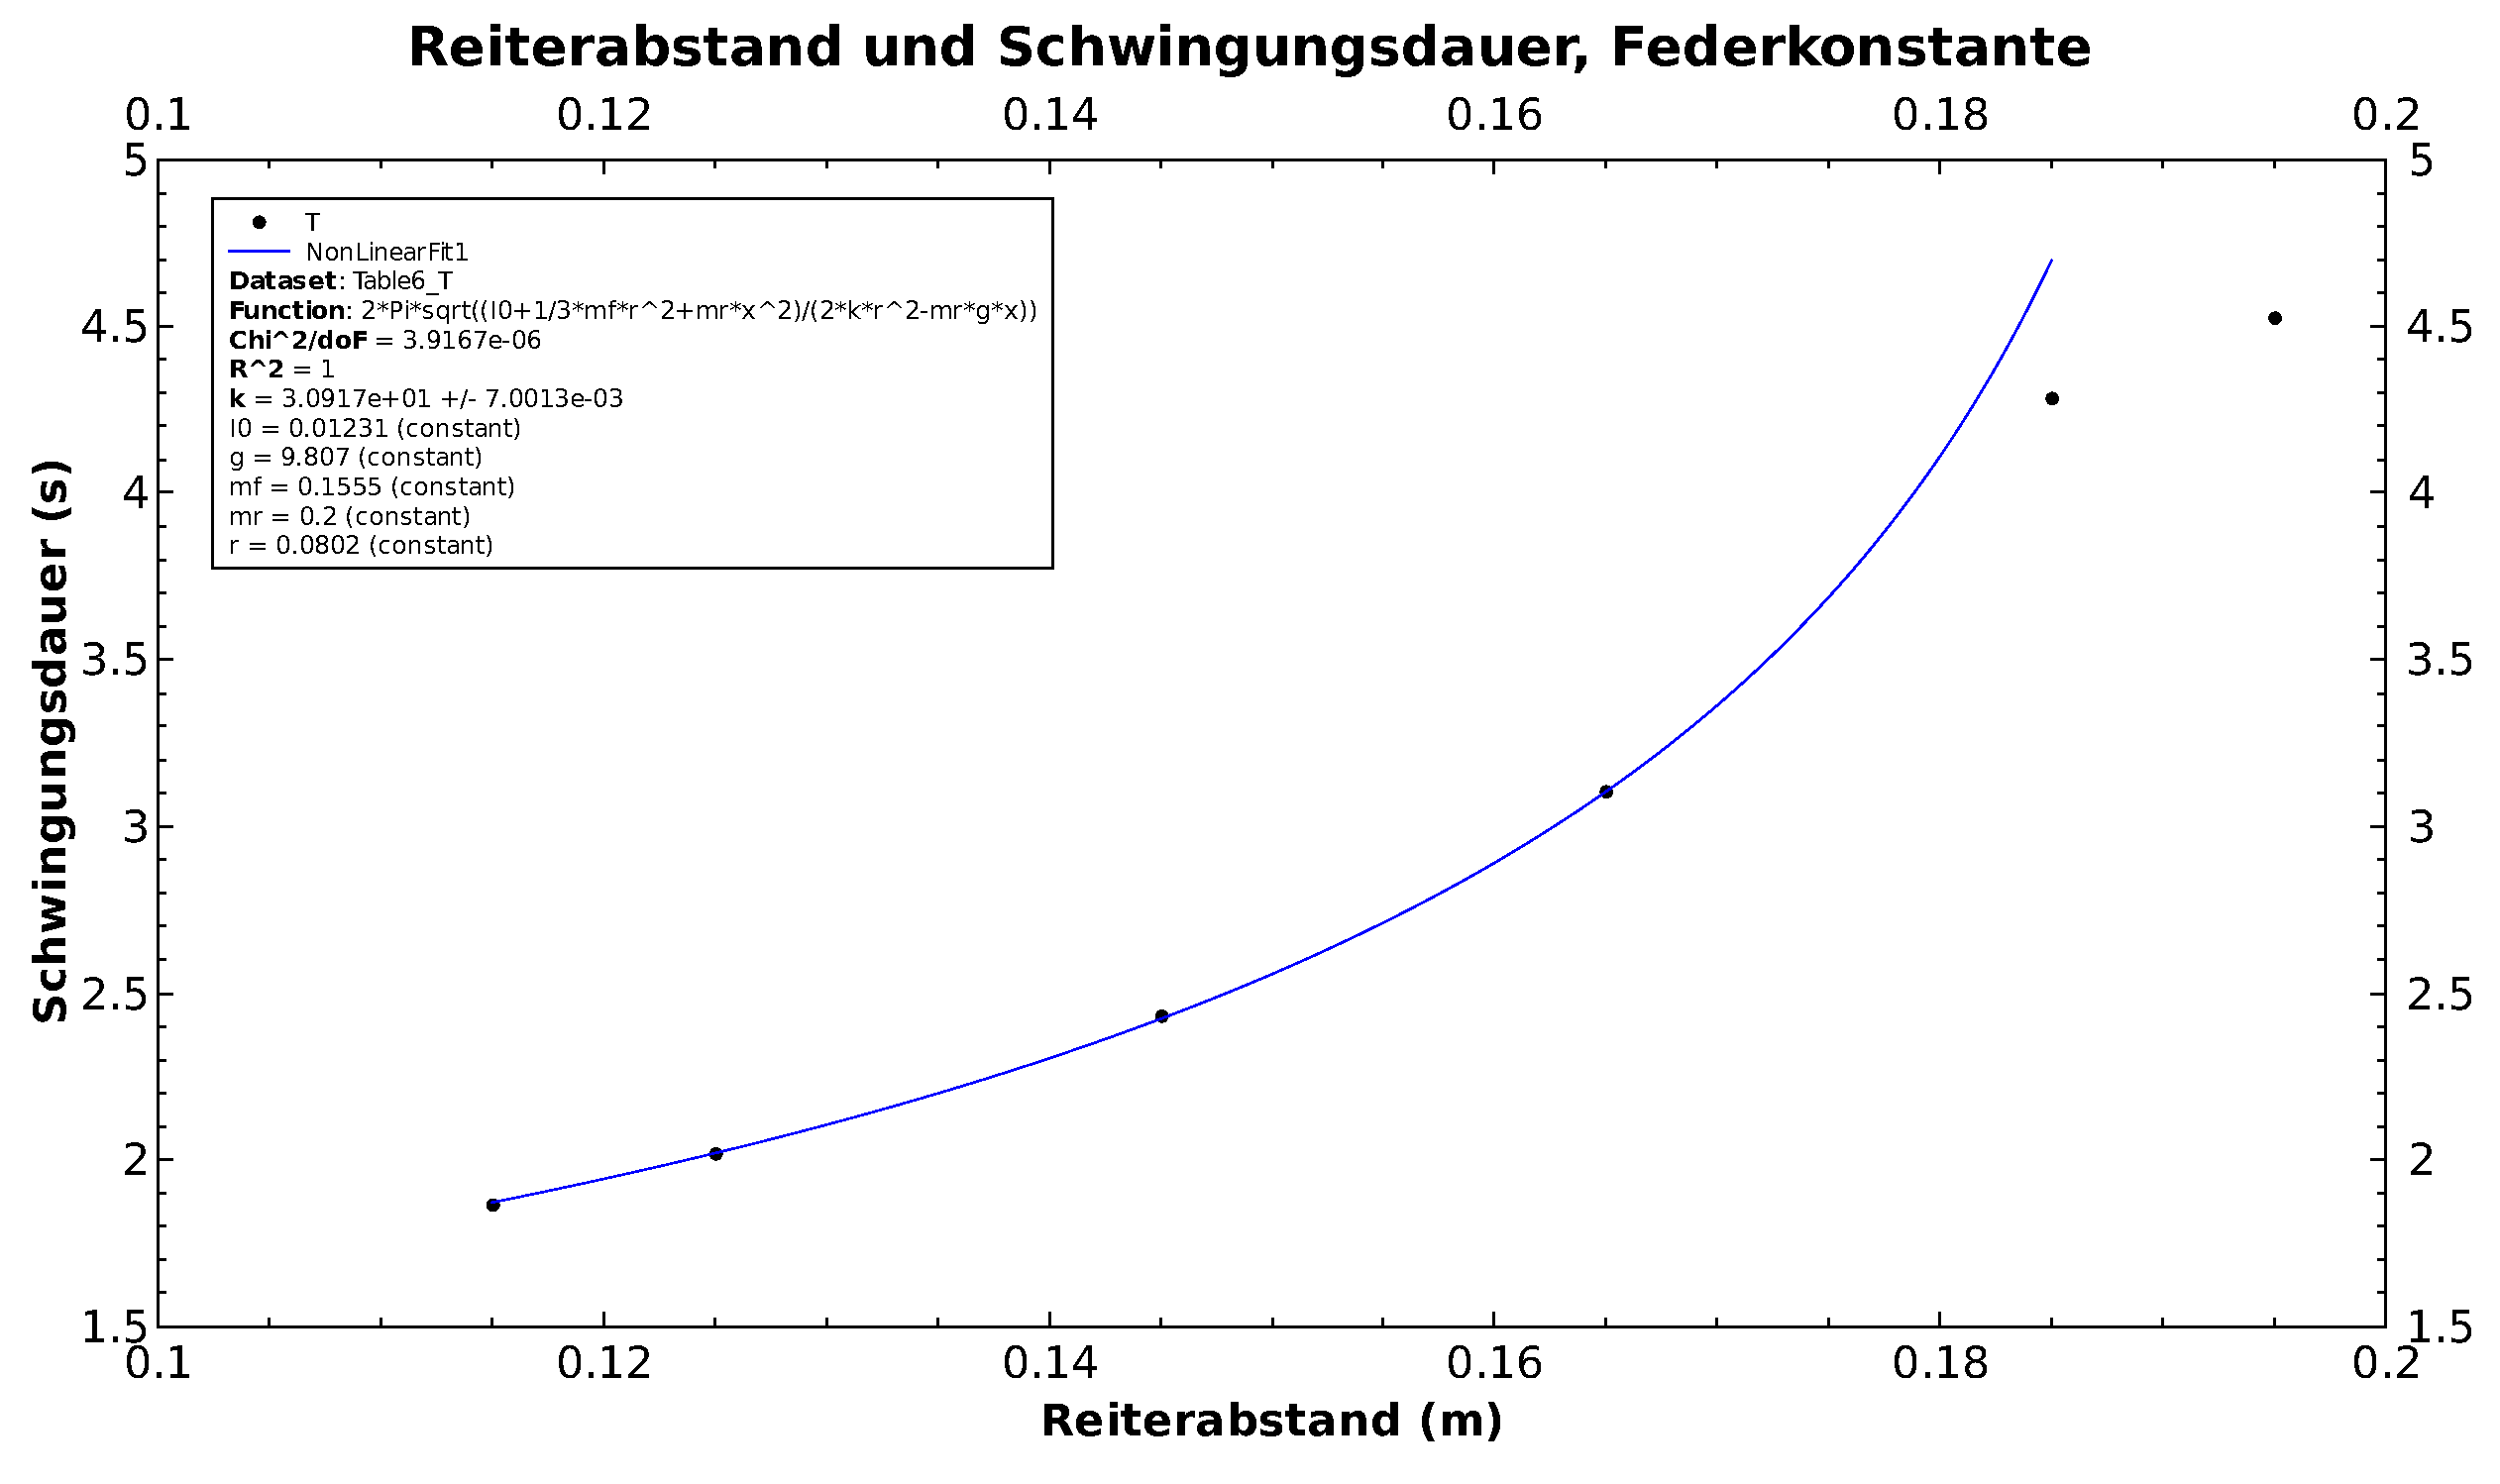
\includegraphics[width=\textwidth]{images/332.pdf}
    \label{fig:pendelKonfigs}
    \caption{%
        Schwingungsdauer in Abh\"angigkeit der Reiterposition beim invertierten Kombipendel unterhalb des kritischen Abstandes. Letzter Messpunkt wurde als Ausreisser behandelt und im Fit nicht ber\"ucksichtigt.
    }
\end{figure}

Die verwendeten Parameter sind
\begin{itemize}
    \item
        $I_0  = \SI[separate-uncertainty = true]{12.311}{\gram\meter\squared}$.
    \item
        $g = \SI{9.807}{\meter\per\second\squared}$
    \item
        $m_{Federn} = \SI{155.5}{\gram}$
    \item
        $m_{Reiter} = \SI{200}{\gram}$
    \item
        $r = \SI{80.2}{\milli\meter}$
\end{itemize}

Gefittet wurde  wiederum f\"ur  die Federkonstante,  was einen  Wert von:

$k = \SI[separate-uncertainty  =  true]{30.917 \pm  0.0070013}{\newton\per\meter}$,

was auch ziemlich nahe beim Wert aus der Versuchsanleitung liegt.

% ---------------------------------------------------------------------------- %
\clearpage
\subsection{Versuch 3.3.3 -- Ruhelagen}
\label{subsec:ruhelagen}
% ---------------------------------------------------------------------------- %


% ---------------------------------------------------------------------------- %
\subsubsection{Reiterposition}
\label{subsubsec:reiterpos}
% ---------------------------------------------------------------------------- %


Auch  mit dem  invertierten Pendel  und dem  Reiter ausserhalb  des kritischen
Abstandes kann  wiederum die  Federkonstante $k$  bestimmt werden. Allderdings
muss hier eine andere Formel verwendet werden:

\begin{equation}
    \frac{\varphi_0}{sin(\varphi_0)} = \frac{a}{a_G} = \frac{q}{p} = \frac{m_{Reiter} \cdot g \cdot a}{2 \cdot k \cdot r^2}
\end{equation}

Wobei $r =  \SI{80.2}{\milli\meter}$, $m_{Reiter} = \SI{200}{\gram}$  und $g =
\SI{9.807}{\meter\per\second\squared}$. $a$  entspricht der  x-Achse, gefittet
wurde \"uber $k$.

\begin{figure}[h!]
    \centering
    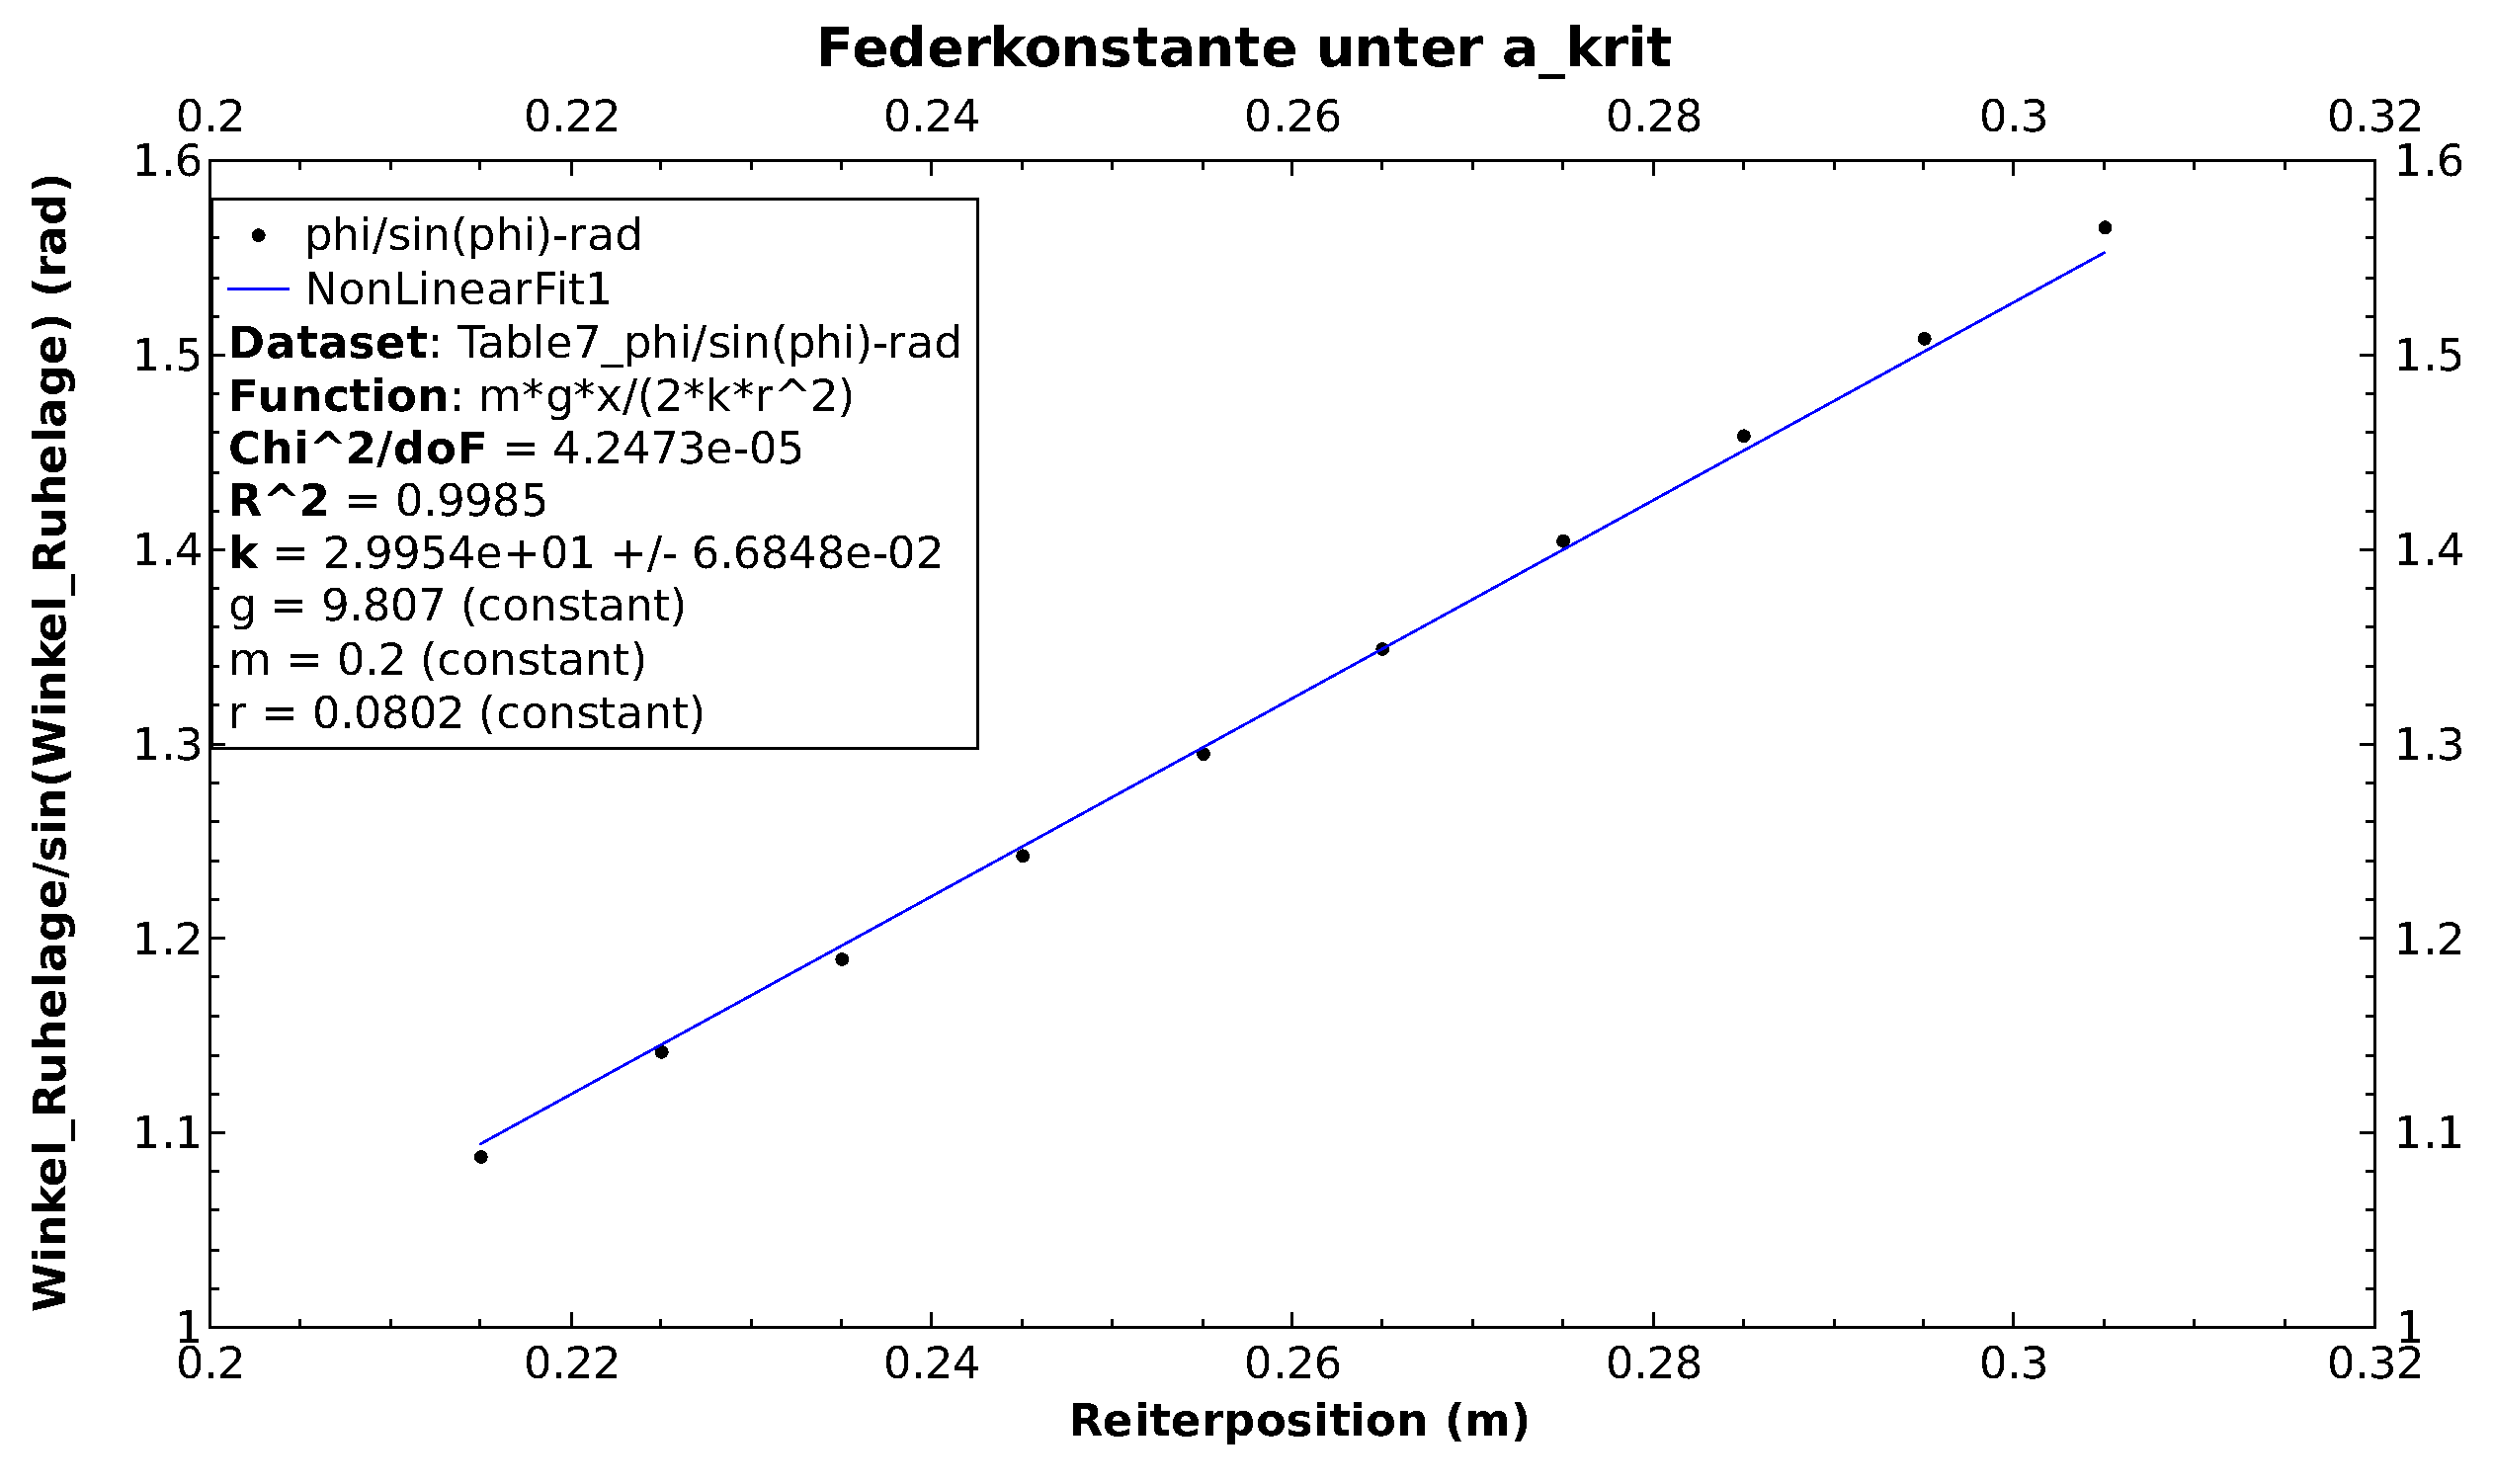
\includegraphics[width=\textwidth]{images/333a.pdf}
    \caption{%
        Bestimmung des Parameters $k$ via Ruhelage, $a>a_{krit}$
    }
    \label{fig:333a}
\end{figure}

Aus dem Fit in Abbildung \ref{fig:333a} erh\"alt man also
$k = \SI[separate-uncertainty  =  true]{29.954 \pm  0.066848}{\newton\per\meter}$.
Auch dieses Ergebnis scheint mir recht zufriedenstellend.


% ---------------------------------------------------------------------------- %
\clearpage
\subsubsection{Schwingungsdauer}
\label{subsubsec:schwingungsdauer}
% ---------------------------------------------------------------------------- %

Zu  guter  letzt  sind  in  Abbildung  \ref{fig:333b}  die  Periodenzeiten  in
Ab\"angigkeit   der  Reiterposition   ausserhalb   des  kritischen   Abstandes
geplotted. Es wurde aber gem\"ass Versuchsanleitung kein Fit ausgef\"uhrt.

\begin{figure}[h!]
    \centering
    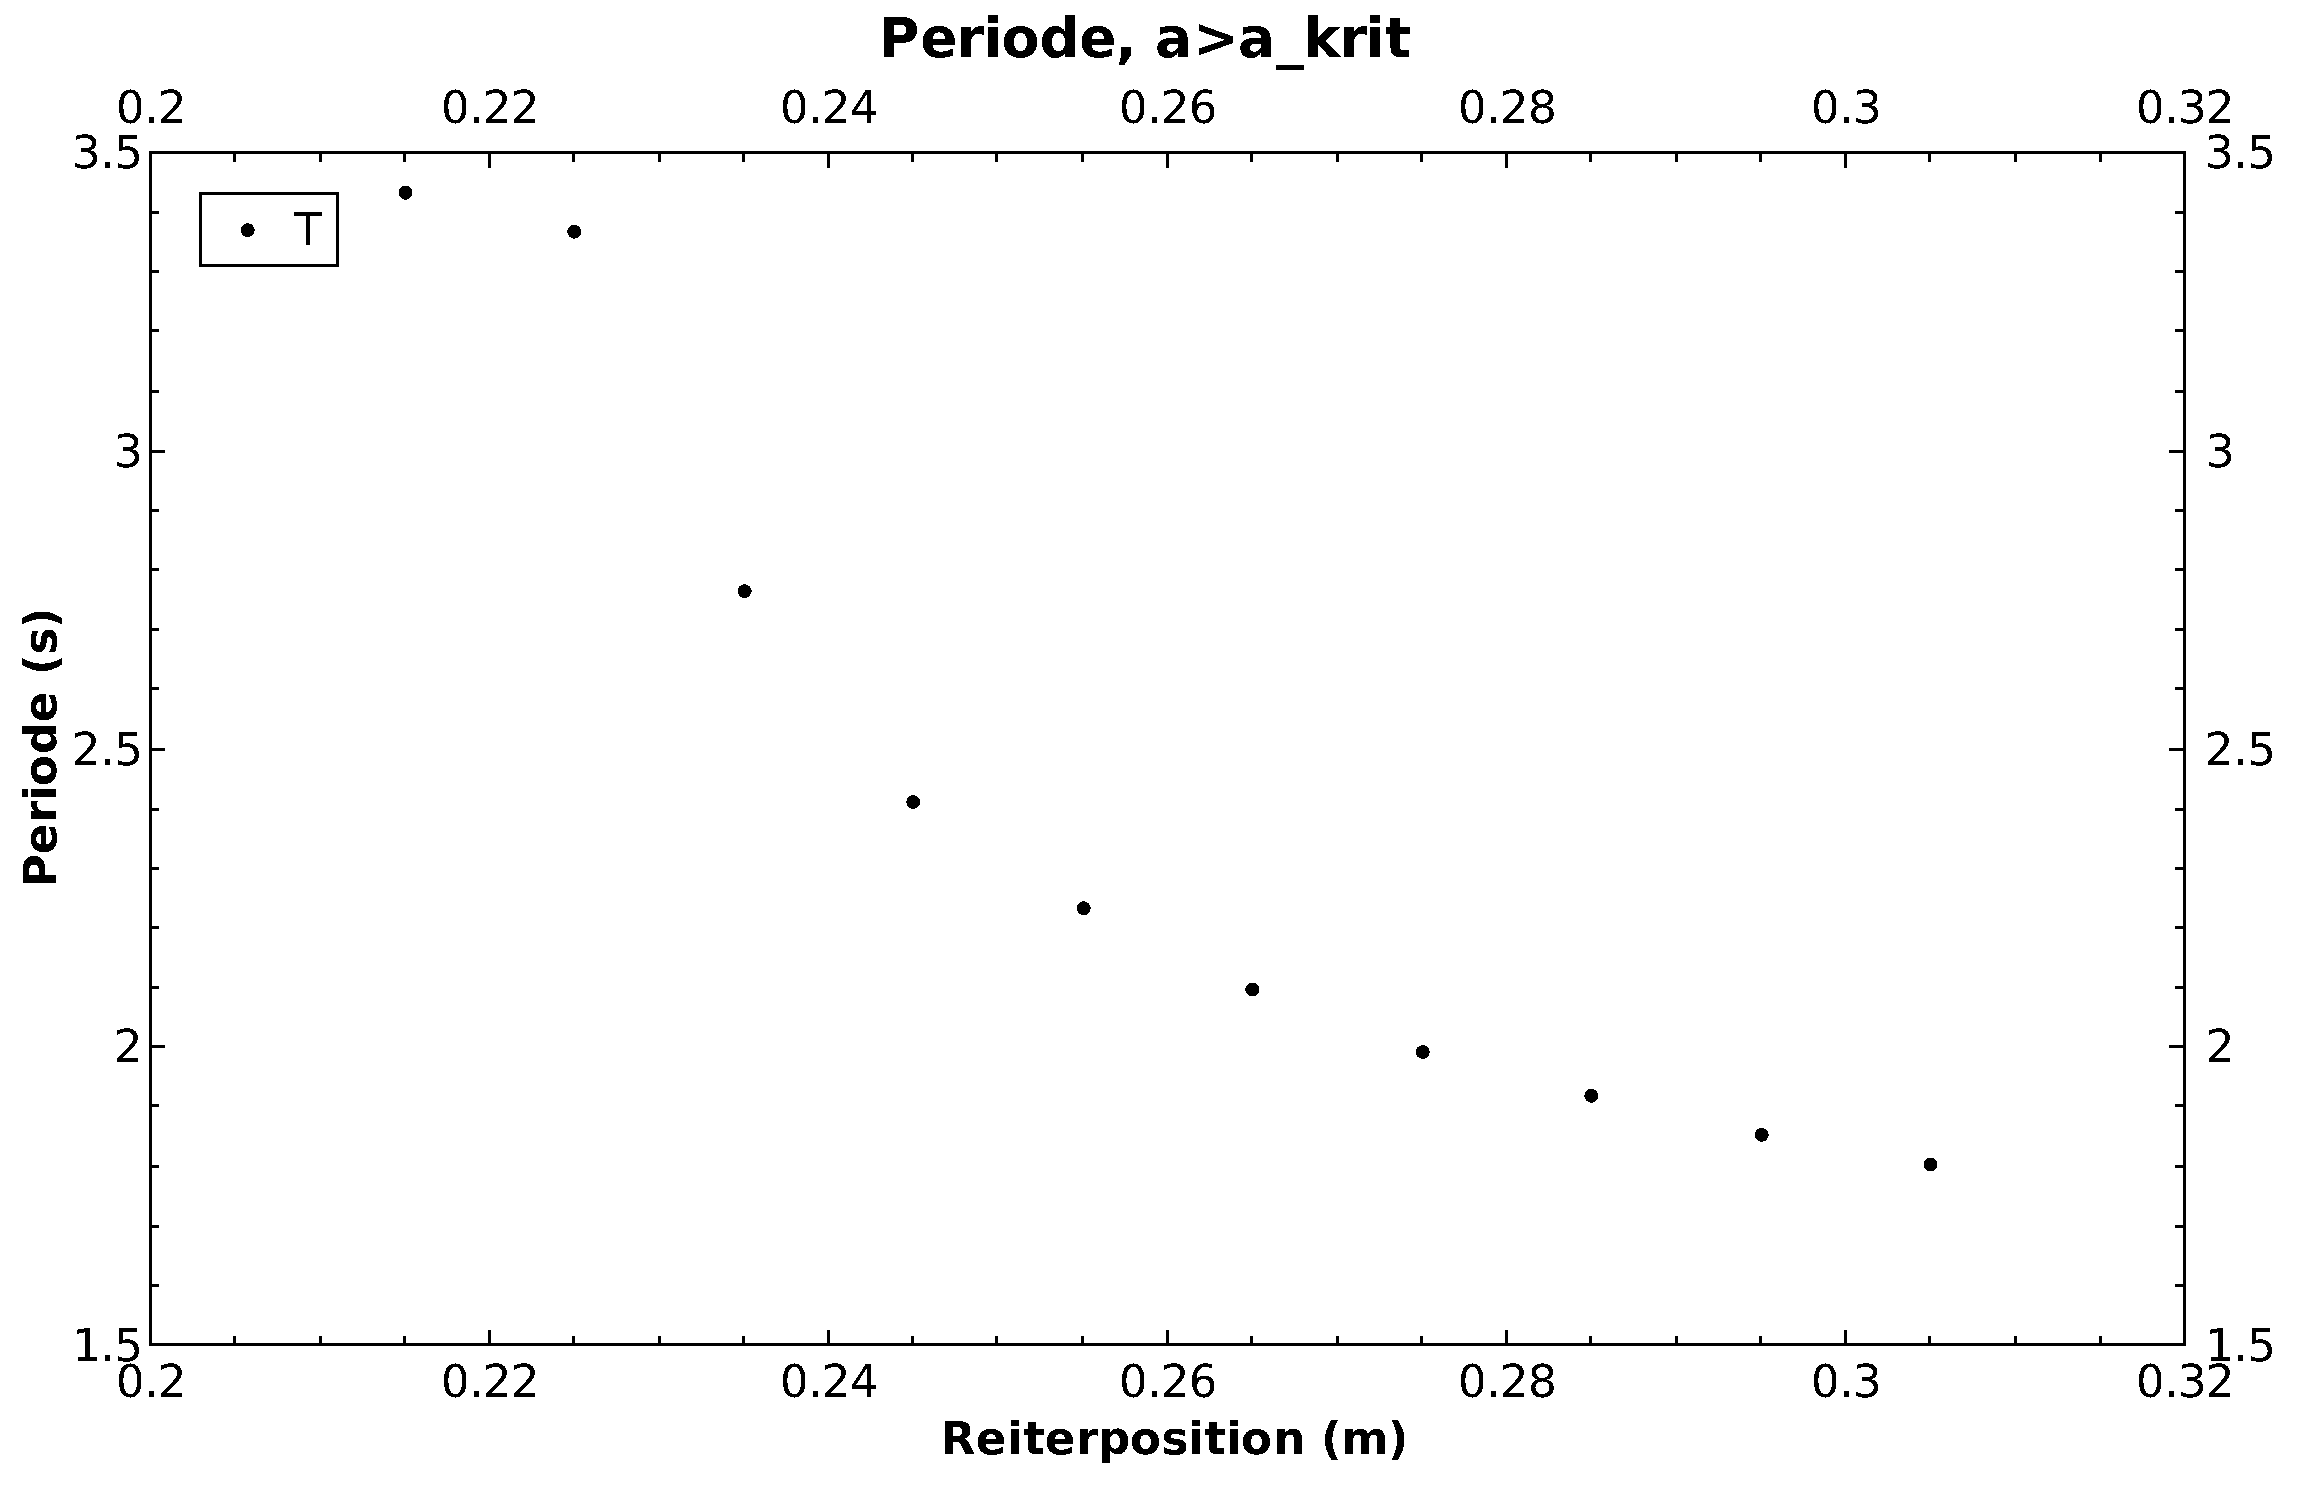
\includegraphics[width=\textwidth]{images/333b.pdf}
    \caption{%
        Periode in Abh\"angigkeit der Reiterposition f\"ur $a>a_{krit}$
    }
    \label{fig:333b}
\end{figure}
